\documentclass{source/Paper}

\begin{document}
    \tableofcontents
    % http://netmedia.zju.edu.cn/compiler
    %https://www.yuque.com/xianyuxuan/coding/compiler

    \newpage
\section{Introduction}

A compiler is a program to translates one language to another.

A Real program language Tiger: Simple and Nontrivial

Two Important Concepts:
\begin{itemize}
    \item Phases(阶段): one or more modules
    \subitem Operating on the different abstract ``languages'' during compiling process
    \item Interfaces(接口)
    \subitem Describe the information exchanged between modules of the compiler
\end{itemize}

\subsection{Modules and Interfaces}

\subsubsection{Modules}
Role: implementing each phase

Advantage: allowing for reuse of the components

\subsubsection{Interfaces}
The data structures: Abstract Syntax, IR Trees and Assem.

A set of functions: The translate interface.

\subsubsection{Phases}
\begin{enumerate}
    \item Lex
    \item Parse
    \item Parsing Actions
    \item Semantic Analysis
    \item Frame Layout
    \item Translate
    \item Canonicalize
    \item Instruction Selection
    \item Control Flow Analysis
    \item Dataflow Analysis
    \item Register Allocation
    \item Code Emission
\end{enumerate}

\subsubsection{Modularization(模块化)}

\subsection{Tools and Software}
Two of the most useful abstractions:
\begin{enumerate}
    \item Context-Free Grammars for parsing
    \item Regular Expressions for lexical analysis
\end{enumerate}

Two tools for compiling:
\begin{enumerate}
    \item Yacc converts a grammar into a parsing program
    \item Lex converts a declarative specification(声明性规范) into a lexical analysis program
\end{enumerate}

\subsection{Data structures for tree languages}

\subsubsection{Intermediate Representations (IR)}
The form of a compiling program: Trees Representation(TR):
\begin{itemize}
    \item The main representation forms
    \item Several node types with different attributes
\end{itemize}

\subsubsection{An example of a program}


\subsubsection{Programming style}
Several conventions for representing tree data structures in C
\begin{enumerate}
    \item Trees are described by a grammar
    \item A tree is described by one or more typedef, each corresponding to a symbol in the grammar.
    \item Each typedef defines a pointer to a corresponding struct.
    \subitem The struct name, which ends in an underscore, is never used anywhere except in the declaration of the typedef and the definition of the struct itself.
    \item Each struct contains a kind fields
    \subitem An enum showing different variants, one of each grammar rule; and a u field, which is a union.
    \item There is more than one nontrivial(value-carraying) symbol in the right-hand side of a rule. The union has a component that is itself a struct comprising these values
    \item %TODO 
\end{enumerate}


\subsubsection{Modularity principle for C programs}
\begin{enumerate}
    \item %TODO 
\end{enumerate}

    \newpage
\section{Lexical Analysis}
To translate a program from one language into another, a compiler first pull it apart and understand its structure and meaning, then put it together in a different way.

\begin{itemize}
    \item The front end(前端): performs analysis
    \item The back end(后端): performs synthesis
\end{itemize}

The analysis is usually broken up into:
\begin{enumerate}
    \item Lexical analysis
    \item Syntax analysis
    \item Semantic analysis
\end{enumerate}

Task of the lexical analyzer:
\begin{enumerate}
    \item Taking a stream of characters
    \item Produces a stream of tokens
    \item Discarding white space and comments
\end{enumerate}

\subsection{Lexical Token}
\subsubsection{A lexical token}
\begin{itemize}
    \item A sequence of characters
    \item A unit in the grammar of a programming language
\end{itemize}

\subsubsection{Token types}
Classification of lexical tokens: A finite set of token types.
\begin{figure}[!htb]
    \centering
    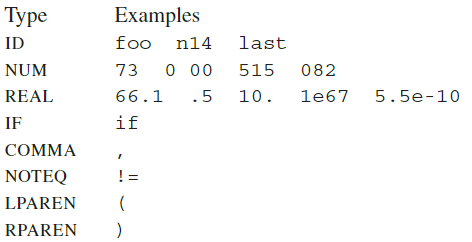
\includegraphics[width=0.42\textwidth]{pic/CP2/Token types}
    \caption{Token types}
\end{figure}

\subsubsection{Non-Tokens}
\begin{figure}[!htb]
    \centering
    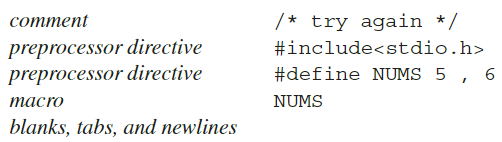
\includegraphics[width=0.42\textwidth]{pic/CP2/Non-Tokens}
    \caption{Non-Tokens}
\end{figure}
The preprocessor deletes the non-tokens.

\subsubsection{An example}
\begin{minted}{c}
float match0(char *s){ /* find a zero */
    if (!strncmp(s, "0.0", 3))
        return 0.;
}
\end{minted}

\begin{minted}{text}
FLOAT ID(match0) LPAREN CHAR STAR ID(s) RPAREN LBRACE 
IF LPAREN BANG ID(strncmp) LPAREN ID(s) COMMA STRING(0.0) COMMA NUM(3) RPAREN RPAREN 
RETURN REAL(0.0) SEMI 
RBRACE EOF
\end{minted}



\subsubsection{An ad hoc lexer}
Any reasonable programming language can be used to implement it. (人和代码有一个能跑就行)

\subsubsection{A simpler and more readable lexical analyzers}
\begin{itemize}
    \item Regular expressions: Specify lexical tokens
    \item Deterministic finite automata: Implementing lexers
    \item Mathematics: Connecting the above two
\end{itemize}

\subsection{Regular Expression}
\subsubsection{Some Concepts}
\begin{itemize}
    \item A language is a set of strings
    \item A string is a finite sequence of symbols (string 没有被赋予意义)
    \item A symbol is taken from a finite alphabet
\end{itemize}

\subsubsection{The notation of regular expressions}
% \begin{itemize}
%     \item Symbol: a
%     \item Alternation: A vertical bar $|$
%     \item Concatenation: operator $\cdot$
%     \item Epsilon: $\epsilon$
%     \item Repetition: ${}^*$
%     \subitem Given a regular expression $M$, its Kleene closure is $M^*$.
%     \subitem A string is in $M^*$ if it is the concatenation of zero or more strings, all of which are in M.
% \end{itemize}

\begin{figure}[!htb]
    \centering
    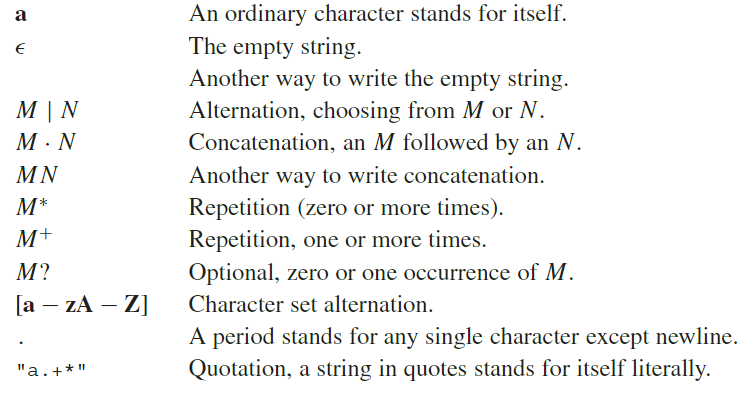
\includegraphics[width=0.42\textwidth]{pic/CP2/Regular expression notation}
    \caption{Regular expression notation}
\end{figure}

\begin{figure}[!htb]
    \centering
    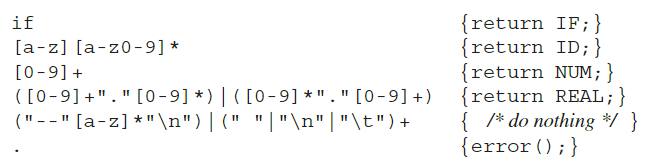
\includegraphics[width=0.42\textwidth]{pic/CP2/Regular expressions for some tokens}
    \caption{Regular expressions for some tokens}
\end{figure}

优先级: ${}^*> \cdot > ||$.

\begin{example}\quad

    \begin{enumerate}
        \item $(0|1)*\cdot0$
        \subitem Binary numbers that are multiples of two
    \end{enumerate}
\end{example}

\subsubsection{Two important disambiguation rules}
These rules are a bit ambiguous.

\begin{enumerate}
    \item Longest match
    \subitem The longest initial substring of the input that can match any regular expression is taken as the next token.
    \item Rule priority
    \subitem The first regular expression that can match determines its token-type
\end{enumerate}

\subsection{Finite Automata}
\subsubsection{A finite automaton}
\begin{definition}[A finite automaton]\quad 
    \begin{itemize}
        \item A finite set of states;
        \item Edges lead from one state to another, and each edge is labeled with a symbol ;
        \item One state is the start state, and certain of the states are distinguished as final states.
    \end{itemize}
\end{definition}

\begin{figure}[!htb]
    \centering
    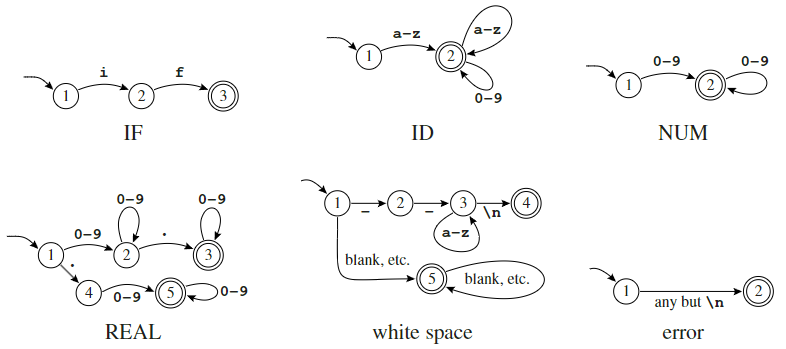
\includegraphics[width=0.42\textwidth]{pic/CP2/Finite automata for lexical tokens.}
    \caption{Finite automata for lexical tokens.}
\end{figure}

\subsubsection{Deterministic Finite Automaton (DFA)}
A DFA accepts or rejects a string as follows: TLDR. 

看计算理论 II.1-6.

\subsubsection{Combined finite automaton}
Using ad hoc method.

\begin{figure}[!htb]
    \centering
    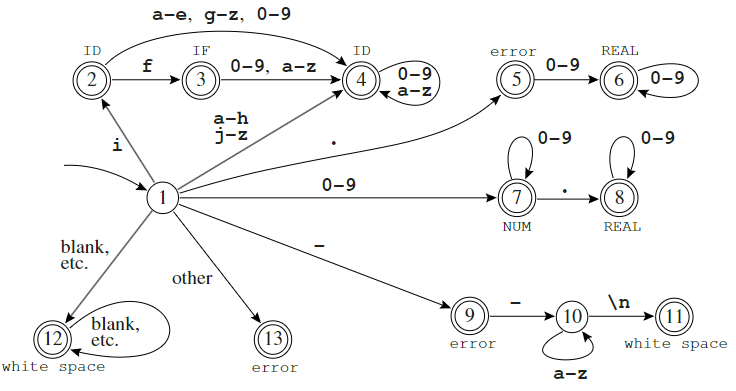
\includegraphics[width=0.42\textwidth]{pic/CP2/Combined finite automaton}
    \caption{Combined finite automaton}
    \label{fig:CDFA}
\end{figure}

\subsubsection{A transition matrix}
Encoding \textbf{Figure} \ref{fig:CDFA}

\subsection{Nondeterministic Finite Automata}
\subsubsection{NFA}
A NFA: 
\begin{itemize}
    \item Have to choose one from the edges to follow out of a state
    \item Have special edges labeled with $\epsilon$
\end{itemize}

\subsubsection{From a RE to an NFA}
The conversion algorithm: (计算理论 III.2 上说这个转换是 naive 的)
\begin{enumerate}
    \item Turning each regular expression into an NFA with a tail (start edge) and a head (ending state).
    \item The rules for translating
\end{enumerate}

\subsubsection{From an NFA to a DFA}
To avoid guesses by trying every possibility at once.

这个计算理论有, II.13.

\subsubsection{The equivalent states}
略
\subsection{Lex: A Lexical Analyzer Generator}
看书
    \newpage
\section{Parsing}
\begin{itemize}
    \item Lexical Analysis: Create sequence of tokens from characters
    \item Parsing: Create abstract syntax tree from sequence of tokens
\end{itemize}

Syntax: the way in which words are put together to form phrases, clauses, or sentences

\begin{itemize}
    \item Input: sequence of tokens from lexer; 
    \item Output: parse tree of the program (But some parsers never produce a parse tree ...)
\end{itemize}

\begin{figure}[!htb]
    \centering
    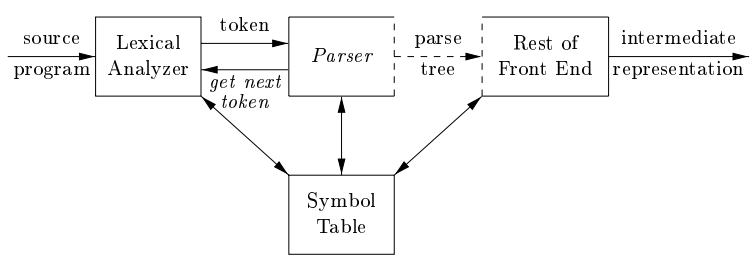
\includegraphics[width=0.42\textwidth]{pic/CP3/compiler.png}
    \caption{compiler}
\end{figure}


\subsection{Context-free Grammars}
\subsubsection{Definition for CFG}
计算理论 IV.1.

\subsubsection{Derivations}
计算理论 IV.2-3

用 CFG 生成 string

\subsubsection{Parse Trees}
计算理论 IV.5

Representing derivations as a tree. Parse trees have meaning. 

\subsubsection{Ambiguous Grammars}
A grammar is ambiguous if the same sequence of tokens can give rise to two or more parse trees.

解决二义性(Ambiguity)的方式就是重写文法. 解决二义性没有通用的方法, 一般都是通过声明 precedence(优先级) 与 associativity(结合性) 来消除文法中的二义性.

\subsubsection{End-Of-File Marker}
Use \$ to represent end of file

\subsection{Predictive Parsing}

\subsubsection{Recursive-Descent Parser}
Each grammar production turns into one clause of a recursive function. 自顶向下分析.

Problem: 预测分析需要每个子表达式的 the first terminal symbol 提供足够的信息来决定生成的是什么.

\begin{definition}[Nullable]
    Non-terminal $X$ is Nullable if $X$ can derive the empty string.
\end{definition}

\begin{definition}[First Sets]
    $First(\gamma)$ is the set of terminals that can begin strings derived from $\gamma$.
    \begin{align*}
        First(X)=\{ t|X\to^*t\alpha \}\cup\{ \epsilon | X\to^*\epsilon \}
    \end{align*}
\end{definition}
即, 如果 $X$ 可以经 0 步或多步推导出以 terminal $t$ 开头的串, 那么 $t$ 属于 ${First}(X)$;如果 $X$ 可以经 0 步或者多步推导出空串, 那么 $\epsilon$ 属于 ${First}(X)$. 

\begin{definition}[Follow Sets]
    $Follow(X)$ is the set of terminals that can immediately follow $X$. That is, $t \in Follow(X)$ if there is any derivation containing $Xt$. This can occur if the derivation contains $XYZt$ where $Y$ and $Z$ both derive $\epsilon$.
    \begin{align*}
        Follow(X)=\{ t|S\to^*\alpha Xt\beta \}
    \end{align*}
\end{definition}

$\epsilon$ 不会出现在 Follow Sets 中. Start Symbol 的 Follow Set 包含文件结束符 \$. 

\begin{algorithm}[H]
    \caption{Compute $First$, $Follow$, and $nullable$}
    \begin{algorithmic}
        \State Initialize $First$ and $Follow$ to all empty sets, and nullable to all false.
        \For{each terminal symbol $t$}
            \State $First(t)\gets \{ t \}$
        \EndFor
        \Repeat
            \For{each production $X\to Y_1Y_2\dots Y_k$}
                \For{each $i$ from $1$ to $k$, each $j$ from $i+1$ to $k$}
                    \If{all the $Y_i$ are nullable}
                        \State $nullable(X)\gets true$
                    \EndIf
                    \If{$Y_1\dots Y_{i-1}$ are all nullable}
                        \State $First(X)\gets First(X)\cup First(Y_i)$
                    \EndIf
                    \If{$Y_{i+1}\dots Y_k$ are all nullable}
                        \State $Follow(Y_i)\gets Follow(Y_i)\cup Follow(X)$
                    \EndIf
                    \If{$Y_{i+1}\dots Y_{j-1}$ are all nullable}
                        \State $Follow(Y_i)\gets Follow(Y_i)\cup First(Y_j)$
                    \EndIf
                \EndFor
            \EndFor
        \Until{$First, Follow$ and nullable didn't change in this iteration.}
    \end{algorithmic}
\end{algorithm}

\subsubsection{Building a Predictive Parser}
\begin{itemize}
    \item $Z\to XYZ | d$
    \item $Y\to c | \epsilon $
    \item $X\to a | Y$
\end{itemize}
\begin{table}[!htb]
    \centering
    \begin{tabular}[c]{cccc}\toprule
        & Nullable & First & Follow \\ \midrule
        $Z$ & no  & $d,a,c$ & \\ \cmidrule{1-1}
        $Y$ & yes & $c$ & $a,c,d $\\ \cmidrule{1-1}
        $X$ & yes & $a,c$ & $a,c,d$\\
        \bottomrule
    \end{tabular}
\end{table}


\subsubsection{Building parsing table}
\begin{itemize}
    \item if $T\in First(s)$ then enter $(X\to s)$ in row $X$, col $T$
    \item if $s$ is Nullable and $T\in Follow(X)$, enter $(X\to s)$ in row $X$, col $T$
\end{itemize}

Build parsing table where row $X$, col $T$ tells parser which clause to execute in function $X$ with next-token $T$:
\begin{table}[!htb]
    \centering
    \begin{tabular}[c]{cccc}\toprule
        & $a$ & $c$ & $d$\\ \midrule
        $Z$ & $Z\to XYZ$ & $Z\to XYZ$ &     \begin{tabular}[c]{@{}l@{}} $Z\to d$ \\ $Z\to XYZ$ \end{tabular} \\ \cmidrule{1-1}
        $Y$ & $Y\to\ $ &     \begin{tabular}[c]{@{}l@{}} $Y\to\ $ \\ $Y\to c$ \end{tabular} & $Y\to\ $ \\ \cmidrule{1-1}
        $X$ &    \begin{tabular}[c]{@{}l@{}} $X\to a$ \\ $X\to Y$ \end{tabular} & $X\to Y$ & $X\to Y$ \\ 
        \bottomrule
    \end{tabular}
\end{table}

\subsubsection{Predictive Parsing: LL(1)}
依据 grammar 构造的 parsing table 没有冲突, 此 grammar 才能被称为 LL(1) grammar.

LL(1): Left-to-right parse, Left-most derivation, 1 symbol lookahead.

In LL(k) parsing table, columns include every k-length sequence of terminals. 

用栈来存储正在生成的 parse tree, 栈顶为 leftmost non-terminal 或即将匹配的 leftmost terminal. 

\begin{example}\quad

    \begin{itemize}
        \item $E\to TX$
        \item $T\to \text{int }Y|(E)$
        \item $X\to +E|\epsilon$
        \item $Y\to *T|\epsilon$
    \end{itemize}
    \begin{table}[!htb]
        \centering
        \begin{tabular}[c]{cccc}\toprule
             & Nullable & First & Follow\\ \midrule
            $E$ & no & $(,\text{int}$ & $),$ \$  \\ \cmidrule{1-1}
            $X$ & yes & $+, \epsilon$ &  $),$ \$ \\ \cmidrule{1-1}
            $T$ & no & $(,\text{int}$ & $+,),$ \$  \\ \cmidrule{1-1}
            $Y$ & yes & $*, \epsilon$ & $+,),$ \$ \\ 
            \bottomrule
        \end{tabular}
    \end{table}

    \begin{table}[!htb]
        \centering
        \begin{tabular}[c]{ccccccc}\toprule
             & int & $*$ & $+$ & $($ & $)$ & \$ \\ \midrule
            $E$ & $TX$ & & & $TX$ & &  \\ \cmidrule{1-1}
            $X$ & & & $+E$ & & $\epsilon$ & $\epsilon$  \\ \cmidrule{1-1}
            $T$ & int $Y$ & & & $(E)$ & &  \\ \cmidrule{1-1}
            $Y$ & & $*T$ & $\epsilon$ & & $\epsilon$ & $\epsilon$  \\ 
            \bottomrule
        \end{tabular}
    \end{table}
    
    \begin{table}[!htb]
        \centering
        % \caption{}
        \begin{tabular}[c]{lll}\toprule
            Stack & Input & Action \\ \midrule
            $E$\$ & $\text{int}*\text{int}$\$ & $TX$\\
            $TX$\$ & $\text{int}*\text{int}$\$ & $\text{int }Y$\\
            $\text{int }YX$\$ & $\text{int}*\text{int}$\$ & terminal\\
            $YX$\$ & $*\text{int}$\$ & $*T$\\
            $*TX$\$ & $*\text{int}$\$ & terminal \\
            $TX$\$ & $\text{int}$\$ & int $Y$ \\
            $\text{int} YX$\$ & $\text{int}$\$ & terminal \\
            $YX$\$ & \$ & $\epsilon$ \\
            $X$\$ & \$ & $\epsilon$ \\
            \$ & \$ & Accept \\
            \bottomrule
        \end{tabular}
    \end{table}
    
\end{example}

\subsubsection{Eliminate left-recursion}
消除左递归
Rewrite the grammar so it parses the same language but the rules are different.

\begin{itemize}
    \item $E\to E+T|T \Rightarrow E\to TE', E'\to +TE'|\epsilon$
    \item $A\to A\alpha | \beta \Rightarrow A\to \beta A', A'\to \alpha A' | \epsilon$
\end{itemize}

\subsubsection{Left Factoring}
提取左因子
\begin{itemize}
    \item $E\to T+E|T \Rightarrow E\to TX, X\to +E|\epsilon$
\end{itemize}

\subsubsection{Error Recovery}
How should error be handled?
\begin{itemize}
    \item Raise an exception and quit parsing
    \item Print an error message and recover from the error
\end{itemize}
This can proceed by deleting, replacing, or inserting tokens

\subsection{LR Parsing}
\subsubsection{Bottom-up Parsing}
自底向上分析.

LL(k) 只看前面 $k$ 个 token.

LR(k): Left-to-right parse, Rightmost derivation, k-token lookahead 可以看到代表输入的全部右侧的生成.

Shift-reduce parsing:
\begin{itemize}
    \item Reduce(规约): token 到 non-terminal
    \item Shift(移进): 右移一位, 考虑下一个 terminal
\end{itemize}

LALR variant: The basis for parsers for most modern programming languages, Implemented in tools such as Yacc.

\begin{figure}[!htb]
    \centering
    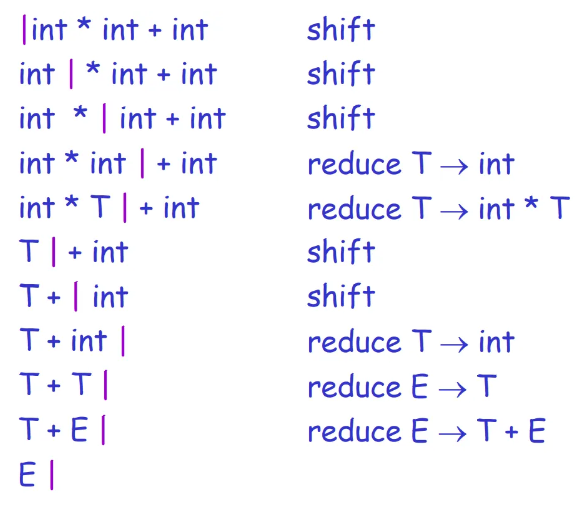
\includegraphics[width=0.309\textwidth]{pic/CP3/lrexp.png}
    \caption{Bottom-up Parsing Example}
\end{figure}

\subsubsection{LR Parsing Engine}
LR parser 使用 DFA 来决定何时 shift/reduce. 具体的:
\begin{enumerate}
    \item 通过 LR items 构造 NFA
    \item NFA 转换为 DFA
    \item DFA 转换为 LR parser table
    \item 依据 LR parser table 决定何时 shift/reduce
\end{enumerate}


一般来说, LR parser table 有以下 elements:
\begin{itemize}
    \item $s_n$: Shift into state $n$
    \item $g_n$: Goto state $n$
    \item $r_k$: Reduce by rule $k$
    \item $a$: Accept
    \item $\ $: Error 
\end{itemize}

LR parser table 具体的使用方式:
\begin{itemize}
    \item $Shift(n)$: Advance input one token; push $n$ on stack.
    \item $Reduce(k)$:
    \begin{enumerate}
        \item Pop stack as many times as the number of symbols on the right-hand side of rule $k$;
        \item Let $X$ be the left-hand-side symbol of rule $k$;
        \item Push $X$ into stack, and look up $X$ to get ``goto $n$''; 
        \item Push $n$ on top of stack.
    \end{enumerate}
    \item $Accept$: Stop parsing, report success
    \item $Error$: Stop parsing, report failure
\end{itemize}

如 \textbf{Figure} \ref{fig:explruse} 所示, stack 需要维护 token 与 state 两个量, 这里使用 (state, token) 对表示. 

\begin{algorithm}[H]
    \caption{LR parser table 使用}
    \begin{algorithmic}
        \State $a$ 表示当前入读的 token. 
        \State $a_{top}, s_{top}$ 分别为 栈顶的 token 与 state.
        \State $T_{(i,a)}$ 表示 parser table 中, state $i$ 行, token $a$ 列 所对应的 element. 
        \Repeat
            \If{$T_{(s_{top}, a)}$ is $s_n$}
                \State PUSH($n, a$)
                \State $a$=GETCHAR()
            \ElsIf{$T_{(s_{top}, a)}$ is $r_k$}
                \State Assume  rule $k$ is $A\to \beta$
                \State POP() $|\beta|$ times
                \State $T_{(s_{top}, A)}$ is $g_n$
                \State PUSH($n, A$)
            \Else
                \State Error
            \EndIf
        \Until{$T_{(s_{top}, a)}$ is accept}
        \State Accept
    \end{algorithmic}
\end{algorithm}

\quad

\quad

\quad

\begin{example}\quad
    
    \begin{enumerate}
        \item $S\to S;S$
        \item $S\to id:=E$
        \item $S\to print(L)$
        \item $E\to id$
        \item $E\to num$
        \item $E\to E+E$
        \item $E\to (S,E)$
        \item $L\to E$
        \item $L\to L, E$
    \end{enumerate}

    \begin{figure}[H]
        \centering
        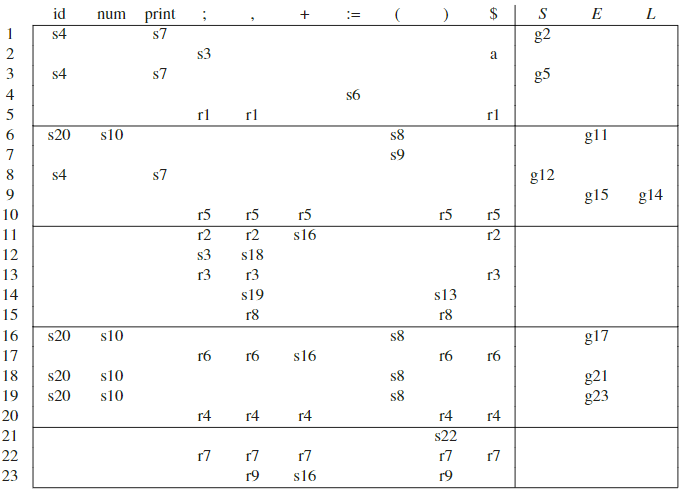
\includegraphics[width=0.42\textwidth]{pic/CP3/lrtable.png}
        \caption{LR parsing table}
    \end{figure}
    
\begin{figure}[H]
    \centering
    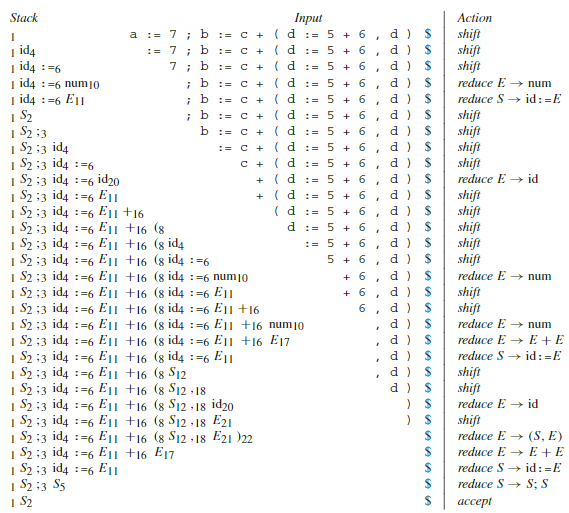
\includegraphics[width=0.42\textwidth]{pic/CP3/Shift-reduce parse of a sentence}
    \caption{Shift-reduce parse of a sentence}
    \label{fig:explruse}
\end{figure}


\end{example}

\subsubsection{LR(0) Parsing}
Making shift/reduce decisions without any lookahead.

% \begin{figure}[!htb]
%     \centering
%     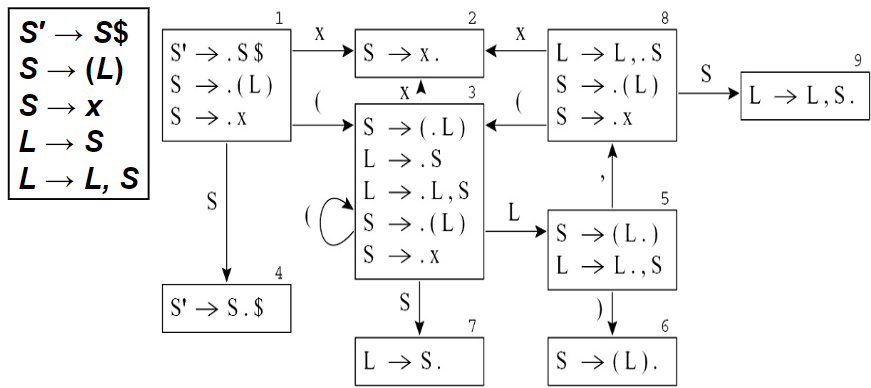
\includegraphics[width=0.42\textwidth]{pic/CP3/LR(0).png}
%     \caption{Items and States}
% \end{figure}

%TODO 完全听不懂, 回去看辅学()

\begin{definition}[LR(0) item]
    A grammar rule, combined with the dot that indicates a position in its right-hand side, is called an item (specifically, an LR(0) item).
\end{definition}

A state is just a set of items.

\begin{example}\label{exp:lr0}
    For grammar
    \begin{enumerate}
        \item $S'\to S$
        \item $S\to (S)S$
        \item $S\to \epsilon$
    \end{enumerate}
    The LR(0) items include:
    \begin{itemize}
        \item $S'\to .S$, $S'\to S.$
        \item $S\to .(S)S$, $S\to (.S)S$, $S\to (S.)S$, $S\to (S).S$, $S\to (S)S.$
        \item $S\to .\epsilon$, $S\to \epsilon.$
    \end{itemize}
\end{example}

LR(0) Item  之间存在一些转换关系:
\begin{itemize}
    \item $X\to .\alpha\beta$, 接受 $\alpha$ 变为 $X\to \alpha . \beta$
    \item 若有 $X\to \gamma T\omega, Y\to \alpha\beta$, 则 $X\to \gamma . Y \omega$ 可以转换为 $Y\to .\alpha \beta$ (因为凑 $X$ 必须先凑 $Y$)
\end{itemize}
通过这些转换关系将 LR(0) items 写为一个 NFA, 然后将 NFA 转换为 DFA. 

% \begin{figure}[!htb]
%     \centering
%     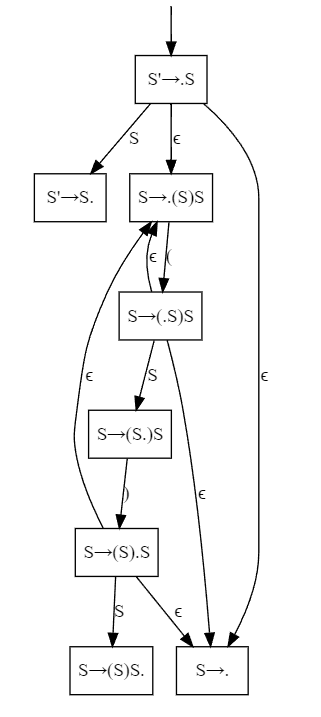
\includegraphics[width=0.22\textwidth]{pic/CP3/expnfa.png}
%     \caption{NFA for \textbf{Example} \ref{exp:lr0}}
% \end{figure}

\begin{figure}[!htb]
    \centering
    \begin{subfigure}{0.22\textwidth}
        \centering
        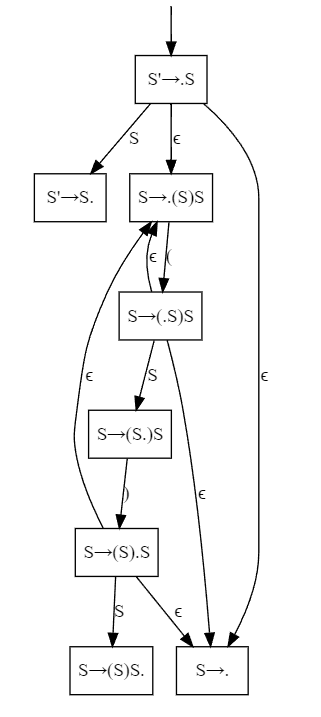
\includegraphics[height=2\textwidth]{pic/CP3/expnfa.png}
        \caption{NFA}
    \end{subfigure}
    \begin{subfigure}{0.22\textwidth}
        \centering
        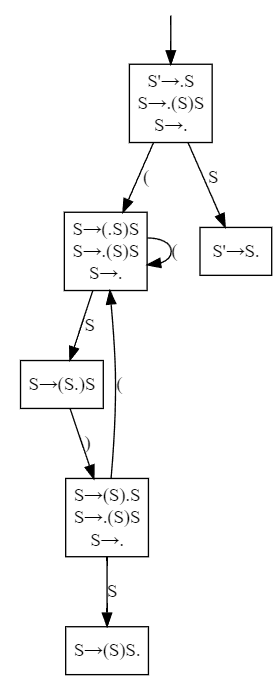
\includegraphics[height=2\textwidth]{pic/CP3/expdfa.png}
        \caption{DFA}
    \end{subfigure}
    \caption{LR(0) NFA and DFA for \textbf{Example} \ref{exp:lr0}}
\end{figure}


然后依据 DFA 与 如下规则:
\begin{itemize}
    \item 对每条 $t$ 是 terminal 的边 $S_i \overset{t}{\rightarrow} S_j$, 令 $T_{(i,t)}$ 为 $s_j$. 其中, $S_i$ 表示状态 $i$,
    \item 对每条 $X$ 是 non-terminal 的边 $S_i \overset{X}{\rightarrow} S_j$, 令 $T_{(i,X)}$ 为 $g_j$.
    \item 对每个包含 $S'\to S.\$ $ 的状态 $i$, 令 $T_{(i,\$)}$ 为 accept.
    \item 对每个包含 $X\to \gamma.$ (结尾带点的规则 $k$) 的状态 $i$, 对每个 terminal $t$, 令 $T_{(i,t)}$ 为 $r_k$.
\end{itemize}

这样就可以构造出 LR(0) Parsing Table, 如 \textbf{Table} \ref{tab:explr0} 所示. 

注意到 $T_{(1,()}, T_{(3,()}, T_{(5,()}$ 出现了冲突, 这三个都属于 shift-reduce conflict. 只有构造出的 LR(0) Parsing Table 没有冲突时, grammar 才能被称为 LR(0) grammar.

\begin{table}[!htb]
    \centering
    \caption{LR(0) Parsing Table for \textbf{Example} \ref{exp:lr0}}
    \label{tab:explr0}
    \begin{tabular}[c]{cccc|c}\toprule
         & ( & ) & \$ & $S$\\ \midrule
        1 & $s_3, r_3$ & $r_3$ & $r_3$ & $g_2$\\ \cmidrule{1-1}
        2 & $r_1$ & $r_1$ & $r_1$, accept & \\ \cmidrule{1-1}
        3 & $s_3, r_3$ & $r_3$ & $r_3$ & $g_4$\\ \cmidrule{1-1}
        4 & & $s_5$ & & \\ \cmidrule{1-1}
        5 & $s_3, r_3$ & $r_3$ & $r_3$ & $g_6$\\ \cmidrule{1-1}
        6 & $r_2$ & $r_2$ & $r_2$ & \\
        \bottomrule
    \end{tabular}
\end{table}


\subsubsection{SLR Parsing}
SLR 中的 S 表示 Simple. SLR Parsing 在 LR(0) 的基础上通过简单的判断尝试解决冲突.

SLR 在构造形如 LR(0) 的 DFA 之上, 还需要计算每个 non-terminal 的 Follow Set. SLR 只对那些下一个符号在对应 non-terminal 的 Follow Set 的情况进行 reduc. 具体更改如下:
\begin{itemize}
    \item 对每个包含 $X\to \gamma.$ (结尾带点的规则 $k$) 的状态 $i$, 对每个 terminal $t\in Follow(X)$, 令 $T_{(i,t)}$ 为 $r_k$.
\end{itemize}

构造出的 SLR Parsing Table, 如 \textbf{Table} \ref{tab:expslr1} 所示.

\begin{table}[!htb]
    \centering
    \caption{SLR Parsing Table for \textbf{Example} \ref{exp:lr0}}
    \label{tab:expslr1}
    \begin{tabular}[c]{cccc|c}\toprule
         & ( & ) & \$ & $S$\\ \midrule
        1 & $s_3$ & $r_3$ & $r_3$ & $g_2$\\ \cmidrule{1-1}
        2 & & & $r_1$, accept & \\ \cmidrule{1-1}
        3 & $s_3$ & $r_3$ & $r_3$ & $g_4$\\ \cmidrule{1-1}
        4 & & $s_5$ & & \\ \cmidrule{1-1}
        5 & $s_3$ & $r_3$ & $r_3$ & $g_6$\\ \cmidrule{1-1}
        6 & & $r_2$ & $r_2$ & \\
        \bottomrule
    \end{tabular}
\end{table}

\subsubsection{LR(1) Parsing}
\begin{definition}
    An LR(1) item consists of a grammar production, a right-hand-side position (represented by the dot), and a lookahead symbol. The idea is that an item ($A \to \alpha.\beta, x$) indicates that the sequence $\alpha$ is on top of the stack, and at the head of the input is a string derivable from $\beta x$.
\end{definition}

LR(1) Item 存在如下两种转化:
\begin{itemize}
    \item $X\to .\alpha\beta, t$ 接受 $\alpha$ 变为 $X\to \alpha . \beta, t$ 
    \item 若有 $X\to \gamma T\omega, Y\to \alpha\beta$, 则对于每个 $t_i\in First(\omega t)$ ($\omega$ 可以是 $\epsilon$),  $X\to \gamma . Y \omega, t$ 可以转换为 $Y\to .\alpha \beta, t_i$
\end{itemize}

\begin{example}\label{exp:lr1}
    对于如下 grammar:
    \begin{itemize}
        \item $S'\to S$
        \item $S \to aAd$
        \item $S \to bBd$
        \item $S \to aBe$
        \item $S \to bAe$
        \item $A \to c$
        \item $B \to c$
    \end{itemize}
    Start Symbol 有 LR(1) Item $S'\to .S, \$ $
    
    \begin{figure}[!htb]
        \centering
        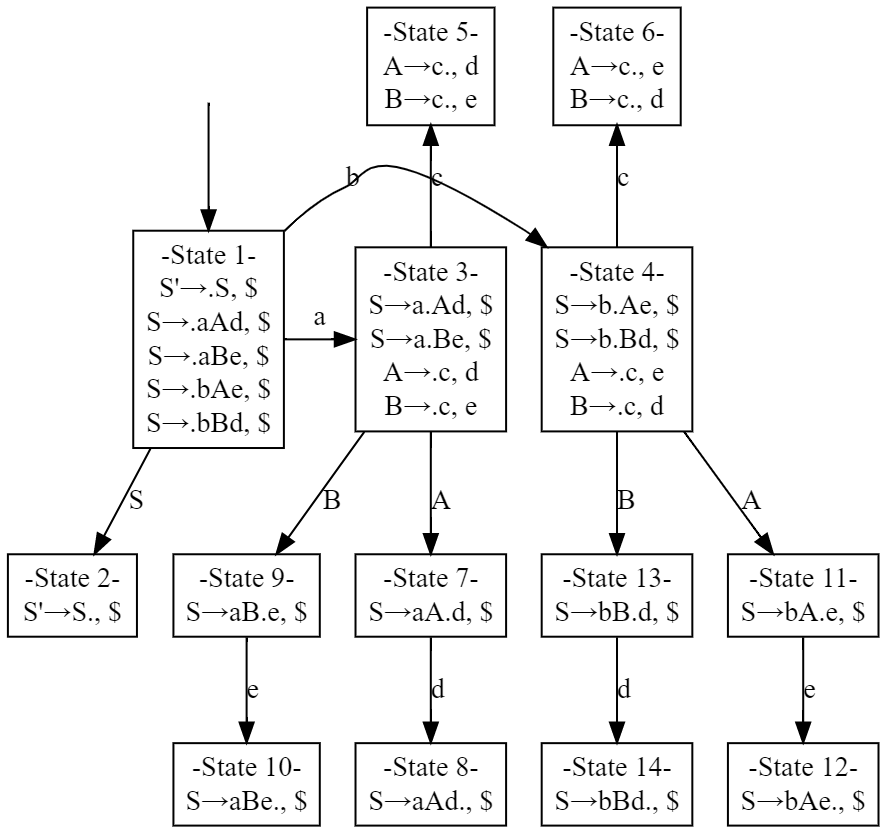
\includegraphics[width=0.42\textwidth]{pic/CP3/explr1dfa.png}
        \caption{LR(1) DFA for \textbf{Example} \ref{exp:lr1}}
        \label{fig:explr1}
    \end{figure}
    
\end{example}

构造 LR(1) Parsing Table 的方式, 也是只基于 LR(0) 更改了 reduce:
\begin{itemize}
    \item 对每个包含 $X\to \gamma.$ (结尾带点的规则 $k$) 的状态 $i$, 对每个 lookahead symbol $t$, 令 $T_{(i,t)}$ 为 $r_k$.
\end{itemize}

\subsubsection{LALR(1) Parsing}
LALR(1)(Look-Ahead LR(1)) 是 LR(1) 的简化版本. 

对于每一个状态, 将其包含的所有 LR(1) items 的第一个分量的集合称为这个状态的核心 (core). 

例如, 对于 \textbf{Figure} \ref{fig:explr1}, 其状态 5 和 6 的核心均为 $\{A\to c., B\to c.\}$. 将这样的具有相同核心的状态进行合并, 通常能够减少许多状态. 

但是, 这有时(虽然很少)也可能引入 reduce-reduce conflict. 不过问题不大. 

\begin{figure}[!htb]
    \centering
    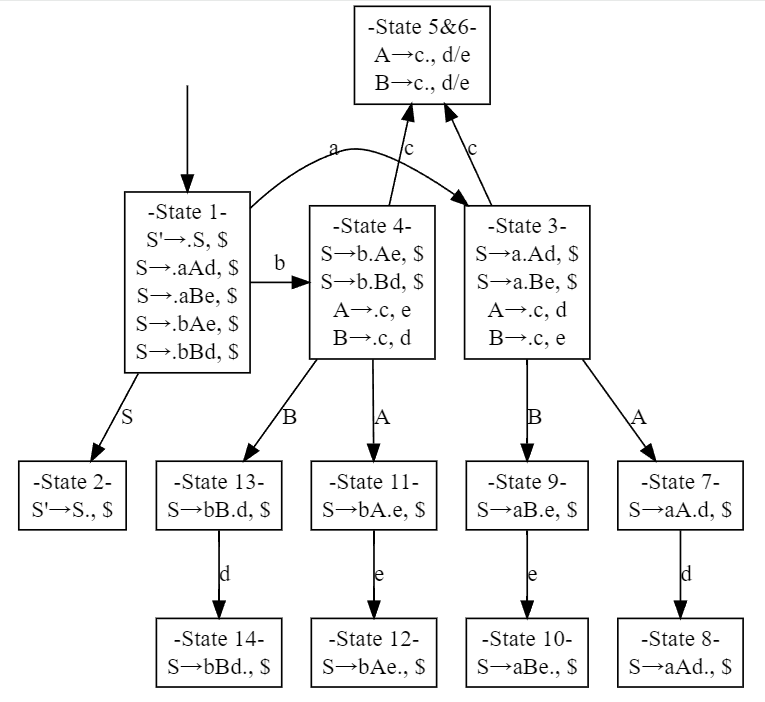
\includegraphics[width=0.42\textwidth]{pic/CP3/explalr1dfa.png}
    \caption{LALR(1) DFA for \textbf{Example} \ref{exp:lr1}}
\end{figure}

\subsubsection{Hierarchy of Grammar Classes}
The relationship between several classes of grammars. 
\begin{figure}[!htb]
    \centering
    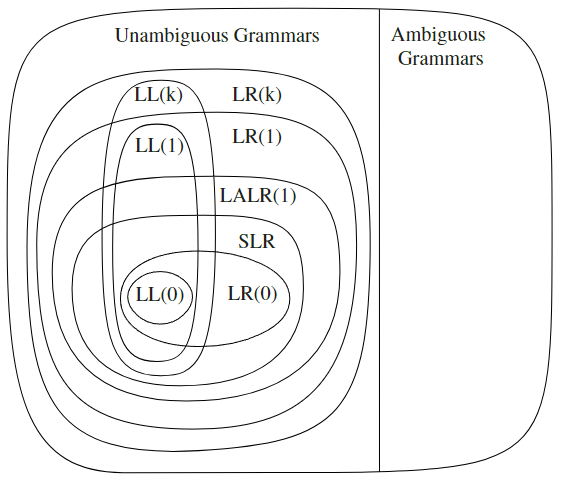
\includegraphics[width=0.309\textwidth]{pic/CP3/A hierarchy of grammar classes.}
    \caption{A hierarchy of grammar classes.}
\end{figure}

\subsection{Using Parser Generators}
\subsubsection{Yacc}
Yacc (``Yet another compiler-compiler''): A classic and widely used parser
generator

A Yacc specification is divided into three sections, separated by \%\% marks:

\begin{minted}{c}
    parser declarations
    %%
    grammar rules
    %%
    programs
\end{minted}

\begin{itemize}
    \item Parser declaration: a list of $N, T$ and so on
    \item Programs: ordinary C code usable from the semantic action
    \item Grammar rules: production of the form
    \subitem \mintinline{c}{exp: exp PLUS exp {semantic action}}  
    \subitem where \mintinline{c}{exp} is a nonterminal producing a right-hand side of \mintinline{c}{exp + exp}, and \mintinline{c}{PLUS} is a terminal symbol (token). The semantic action is written in ordinary C and will be executed whenever the parser reduces using this rule.
\end{itemize}

\begin{example}
    For grammar
    \begin{enumerate}
        \item $P \to L$
        \item $S \to id := id$
        \item $S \to$ while $id$ do $S$
        \item $S \to$ begin $L$ end
        \item $S \to$ if $id$ then $S$
        \item $S \to$ if $id$ then $S$ else $S$
        \item $L \to S$
        \item $L \to L ; S$
    \end{enumerate}

    \begin{minted}{c}
%{
int yylex(void);
void yyerror(char *s) { EM_error(EM_tokPos, "%s", s); }
%}
%token ID WHILE BEGIN END DO IF THEN ELSE SEMI ASSIGN
%start prog
%%
prog: stmlist
stm : ID ASSIGN ID
    | WHILE ID DO stm
    | BEGIN stmlist END
    | IF ID THEN stm
    | IF ID THEN stm ELSE stm
stmlist : stm
        | stmlist SEMI stm
    \end{minted}
    
\end{example}

\subsubsection{Conflicts}
\begin{itemize}
    \item shift-reduce conflict: Resolved using shift by default in Yacc
    \item reduce-reduce conflict: Resolved using the rule appears early in the grammar
\end{itemize}

\subsubsection{Precedence Directives}
Ambiguous grammars are still be useful if finding ways to resolve the conflict.

Yacc uses precedence directives to resolve this class of shift-reduce conflicts

\subsection{Error Recovery}
\subsubsection{Recovery Using the Error Symbol}
Local error recovery mechanisms.

If a syntax error is encountered in the middle of an expression, the parser should skip to the next semicolon or right parenthesis(called synchronizing tokens) and resume parsing.

error is considered a terminal symbol. When the LR parser reaches an error state, it takes the following actions:
\begin{enumerate}
    \item Pop the stack (if necessary) until a state is reached in which the action for the error token is shift.
    \item Shift the error token.
    \item Discard input symbols (if necessary) until a lookahead is reached that has a nonerror action in the current state.
    \item Resume normal parsing.
\end{enumerate}

\subsubsection{Global Error Repair}
Global error repair: finds the smallest set of insertions and deletions that would turn the source string into a syntactically correct string, even if the insertions and deletions are not at a point where an LL or LR parser would first report an error.

Burke-Fisher error repair: single-token insertion, deletion, or replacement at every point that occurs no earlier than $K$ tokens before the point where the parser reported the error.
    \newpage
\section{Overview of Semantic Analysis}

\subsection{Abstract Parse Trees}
这种方法限制编译器按照解析程序的顺序来分析程序.

parse tree(解析树) 从 semantic 中分离 issues of syntax(parsing), 并让编译器后期可以遍历它. 
\begin{itemize}
    \item Concrete parse tree: 代表了源码的 concrete syntax. 从技术上讲, 对于输入的每个 token 只有一个 leaf, 对于 parse 中减少的每个语法规则只有一个内部节点. 但其中的标点符号是冗余信息. 
    \item Abstract parse tree/Abstract syntax tree: abstract syntax 表达了源码的 phrase structure, 在没有任何语义解释下解决所有 parsing 问题. 
\end{itemize}
一般是语义分析 concrete syntax 然后构建 abstract syntax tree.

\subsubsection{Positions}
%TODO 摸了, 似乎不考(虽然期中涉及到但没写出来也没扣分)

\subsection{Symbol Table}
\begin{definition}
    A symbol table is a data structure that tracks the current bindings of identifiers
\end{definition}


\begin{code}
    \caption{A Fancier Symbol Table}
    \begin{minted}{c++}
        enter_scope()   // start a new nested scope
        find_symbol(x)  // finds current x (or null)
        add_symbol(x)   // add a symbol x to the table
        check_scope(x)  // true if x defined in current scope
        exit_scope()    // exit current scope
    \end{minted}
\end{code}

局部变量都有一个作用域(scope), 变量仅在自己的作用域中可见. 

环境是由绑定(binding)组成的集合, 指标识符和含义之间的一种映射关系, 用箭头表示. e.g. $\{g\to string\}$, $\{a\to int\}$

\subsubsection{Imperative(命令式)}
\begin{itemize}
    \item 实现: bucket list(hash table)
\end{itemize}
插入 identifiers 时插入到头部, 在退出 scope 时方便 pop. 

\subsubsection{Functional(函数式)}
\begin{itemize}
    \item 实现: 可持久化二叉搜索树(persistent BST)
\end{itemize}
使用可持久化来控制 scope
    \newpage
\section{Activation Record}
\subsection{Stack Frame(栈帧)}
\begin{definition}
    栈中存放函数的局部变量/参数/返回地址/临时变量的这片区域为该函数的活动记录 (activation record) 或栈帧(stack frame).
\end{definition}
\begin{figure}[!htb]
    \centering
    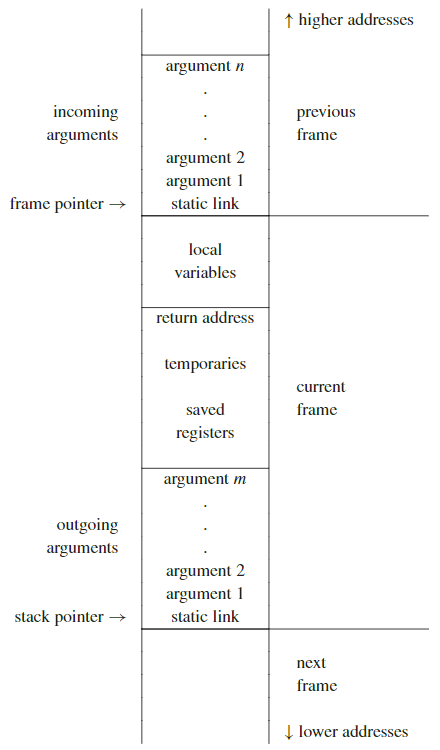
\includegraphics[width=0.319\textwidth]{pic/CP678/a typical stack frame layout.png}
    \caption{a typical stack frame layout}
\end{figure}
\begin{itemize}
    \item incoming arguments: 是前一个帧的一部分, 但其与 frame pointer 的偏移量已知.
    \item return address: 由 CALL 指令创建, 告知完成此函数后需要返回何处.
    \item local variables: 一些在帧中, 一些在寄存器上. 在寄存器与帧中临时空间之间移动.
\end{itemize}

\subsection{Frame Pointer}
指向当前帧的指针,一般是上一个 sp;有些栈帧 会 分 配 一 个 寄 存 器 存fp; 虚寄存器: fp=sp+size(frame). 

帧指针的变化:一个函数 $g$ 调用 $f$ 时,
\begin{enumerate}
    \item sp 指向g 传给 f 的第一个参数
    \item f 分配栈帧(sp-栈帧大 小)
    \item 进入 f 时旧的 sp 变成当前帧指针;fp 旧值被保存到栈帧内,新的帧指针变成旧 sp
    \item f 退出时把 fp 拷贝给 sp,再取回原先保存的 fp 即可.
\end{enumerate}

\subsection{Parameter Passing}
现代计算机传参约定:前 $k$($k=4$ or $k=6$, typically) 个参数放在寄存器里传递,剩余在储存器传递.

寄 存 器 传 参 的 方 法 (4 种 ):
\begin{enumerate}
    \item 不 给 叶 过 程 (leaf procedure)分配栈帧 . 绝大多数过程都是叶过程, 不分配栈帧能节省很多开销.
    \subitem  叶 过 程: 不调用其他过程的过程
    \item 过 程 间 寄 存 器 分 配 (interprocedural register allocation): 先分析代码中全部的函数, 然后再根据分析分配寄存器
    \item 若变量 $x$ 不再被使用, 可以直接写其寄存器, 不需要再保存 $x$ 到栈帧中. 
    \item  寄 存 器 窗 口 技 术 (register windows): 每个函数调用分配一组新的寄存器, 无需内存传输.
\end{enumerate}

\subsection{Frame-Resident Variables}
一般来说局部变量和中间结果会放到寄存器中,以下情况需要将变量储存到栈帧内(memory): 
\begin{enumerate}
    \item 变 量 传 地 址 / 引 用 (passed by reference) 
    \item 被嵌套在 当 前 过 程 的 函 数 调 用(nested accessed) 
    \item 太大 了 放 不 下 (too big to fit)
    \item 变量是数组
    \item 有特殊用途的变量(传参等) 
    \item 存在过多的临时变量和局部变量(溢出 spill)
\end{enumerate}

在以下情况, 称变量为逃逸(escape):
\begin{enumerate}
    \item 传 地 址 
    \item 被取地址
    \item 被内层嵌套函数访问
\end{enumerate}


\subsection{Static Link}
静态链本质是指向上一层嵌套层级的栈帧的指针.内层嵌套函数调用外层定义的变量需要用到静态链,否则无法寻址.

其他访问外层变量的方法:
\begin{enumerate}
    \item 嵌套层次显示表(display):一个全局数组,位置 i 存放最近一次的,静态嵌套深度为 i的过程的栈帧. 是管理静态链的全局数组(不是栈指针) 
    \item $\lambda$ 提升(lambda shifting):内层函数访问的外层声明变量,会作为函数参数传给内层嵌套函数.
\end{enumerate}

注意:静态链层级是函数的嵌套深度(函数之间),不是递归调用的深度(函数自己),两者不同概念

\newpage
\section{Translation to Intermediate Code}
intermediate represent(中 间 表 示): 抽象的机器语言,链接前端和后端,解决了高级语言和目标机器汇编语言之间的转化.

\begin{itemize}
    \item 前端(front end):词法分析,语法分析,语义分析,翻译成中间代码
    \item 后端(back end):IR 优化, 翻译成机器语言.
\end{itemize}

\subsection{Intermediate Representation Trees}
\subsubsection{Tree Operator}

Expressions(T\_exps): 
\begin{itemize}
    \item CONST($i$): 整 型 常 数 
    \item NAME($n$): 符 号 常 数 
    \item TEMP($t$): 临 时 变 量 
    \item BINOP($o, e_1, e_2$):对操作数 $e_1,e_2$ 的 二 元 操 作 
    \item MEM($e$):作为 MOVE 操作的左子式时表示对储存器 $e$ 地址的存入;其他位置表示读取该地址的内容 
    \item CALL($f,l$):过程调用 
    \item ESEQ($s,e$): 先计算语句 s 形成副作用,然后计算 $e$ 违该表达式的值 
\end{itemize}

Statements(T\_stm):
\begin{itemize}
    \item MOVE(TEMP $t, e$): 计算 $e$ 的值然后存到临时变量 $t$ 中
    \item MOVE(MEM($e_1$),$e_2$):计算 $e_2$ 的值然后存入到 $e_1$ 作为地址的内存中 
    \item JUMP($e$,$labs$):跳转到 $e$ 地址 或 者 $labs$ 为 label 的 地 址
    \item CJUMP($o,e_1,e_2,t,f$): 依 次 计 算 $e_1$ 和 $e_2$, 生成值 $a,b$;然后用比较运算符操作 $aob$,如果结果为 true 跳到 $t$,反之跳转到 $f$; 
    \item SEQ($s_1,s_2$):语句 $s_1$ 后 面 跟 $s_2$
    \item LABEL($n$):定会一名字后的常数值为当前机器代码的地址.
\end{itemize}


\subsection{Translation into Trees}
\subsubsection{Kinds of Expressions}
\begin{itemize}
    \item Ex 代表 expression
    \item Nx 代表无结果的 statement
    \item Cx 代表条件分支, 可能跳转到 true label 或 false label.
\end{itemize}

对于 CJUMP 和 JUMP 语句,还 不知道 label 的具体值,需要 使用两张表: 
\begin{itemize}
    \item 真值标号回填表 (true patch list)
    \item 假值标号回填表 (false patch list)
\end{itemize}

\subsubsection{Variables}
\begin{itemize}
    \item Simple variables: 
    \subitem MEM(BINOP(PLUS, TEMP $fp$, CONST $k$))
    \item Following static links:
    \subitem MEM(+(CONST $k_n$, MEM(+(CONST $k_{n-1}$, $\dots$ MEM(+(CONST $k_1$, TEMP $fp$))$\dots$))))
    \item Array variables: 
    \subitem MEM(+(MEM($e$), BINOP(MUL, $I$, CONST $W$)))
\end{itemize}

\subsubsection{Conditionals}
e.g. if $x<5$ then $a>b$ else 0, \\
$x<5$ translates into Cx($s_1$), $a>b$ translates into Cx($s_2$)

SEQ($s_1$($z$,$f$), SEQ(LABEL $z$, $s_2$($t$,$f$)))

\subsubsection{Loops}
\begin{itemize}
    \item while
    \begin{minted}{text}
    test:
        if not(condition) goto done
        body
        goto test
    done:
    \end{minted}
    
    \item for
    \begin{minted}{text}
    for i:=lo to hi         let var i:=lo
        do body                 var limit:=hi
                            in while i<=limit
                                do(body; i:=i+1)
                            end
    \end{minted}
    
\end{itemize}
\subsubsection{Function Call}
CALL(NAME $l_f$, [$sl, e_1, e_2,\dots, e_n$])

$l_f$ is the label for $f$, $sl$ is the static link

\subsection{Declarations}
变量声明将会在 frame 中额外保留部分空间;函数声明会在 Tree code 中保留一个新的 fragment.

变量的初值会被转换成一个 Tree 表达式,transDec 返
回一个 Tr\_Exp,这个 Tr\_Exp 应当包含完成赋初值的
赋值表达式;如果对函数和类型声明施加 transDec,
结果将会得到 Ex(CONST(0))这样的空操作

函数被翻译为入口处理代码(prologue),函数体(body)和出口处理函数(epilogue)组成的汇编语言代码.

入口包含:
\begin{enumerate}
    \item 声明一个函数开始的伪指令(pseudo-instructions)
    \item 函数名 label 的定义
    \item 调整栈指针的一条指令,用于分配新的栈帧
    \item 将逃逸(escaping)参数保存至栈帧的指令,以及将非逃逸参数传送的新临时寄存器指令
    \item 保 存  此 函 数 用 到 的 caller-save 寄存器(包括返回地址寄存器)
\end{enumerate}

本体:
\begin{enumerate}[start=6]
    \item 函数体
\end{enumerate}

出口包含:
\begin{enumerate}[start=7]
    \item 将返回值传送至专用于返回结果的寄存器 
    \item 用 于 恢 复 callee-save 的寄存器取数指令
    \item 恢 复 栈 指 针 , 释 放 栈 帧
    \item return 指令
    \item 声明函数结束的伪指令
\end{enumerate}


\newpage
\section{Basic Blocks and Traces}

\subsection{Canonical Trees(规范树)}
\subsubsection{Definition}
\begin{definition}
    A canonical trees have these properties:
    \begin{enumerate}
        \item No SEQ or ESEQ
        \item The parent of each CALL is either EXP($\dots$) or MOVE(TEMP $t$, $\dots$).
    \end{enumerate}
\end{definition}

Why?
\begin{enumerate}
    \item CJUMP 能够跳转到两个标号的任意一个,但实际的是条件为假时跳转到下一条
    \item ESEQ 会使得子树的不同计算顺序产生不同结果
    \item 表达式使用 CALL 会有计算顺序不同的问题
    \item CALL 的嵌套调用(作为另一个 CALL 的参数)会出问题,覆盖存放返回值的寄存器的值
\end{enumerate}


重写流程:
\begin{enumerate}
    \item 一棵树重写成规范树 
    \item 将树分组合成不含转移和标号的基本块(basicblock)集合 
    \item 对基本块 进行 排 序 形 成 一 组 轨 迹(trace);每一个 CJUMP 后就是其 false 标号
\end{enumerate}

\subsubsection{Transformations on ESEQ}
\begin{enumerate}
    \item ESEQ($s_1$, ESEQ($s_2$,$e$)) $\to$ ESEQ(SEQ( $s_1,s_2$), $e$) 
    \item BINOP($op$,ESEQ($s$,$e_1$), $e_2$) $\to$ ESEQ(BINOP($op$,$e_1$, $e_2$)) 
    \subitem MEM(ESEQ($s$,$e_1$)) $\to$ ESEQ( $s$, MEM($e_1$)) 
    \subitem JUMP(ESEQ($s$, $e_1$)) $\to$ SEQ($s$,JUMP($e_1$)) 
    \subitem CJUMP(op,ESEQ($s$,$e_1$),$e_2$,$l_1,l_2$)\\
    $\to$ SEQ($s$, CJUMP($op$, $e_1$, $e_2$, $l_1,l_2$)) 
    \item BINOP(op,$e_1$, ESEQ(s,$e_2$)) \\
    $\to$ ESEQ(MOVE (TEMP t, $e_1$), ESEQ(s, BINOP(op, TEMP t, $e_2$))) 
    \subitem CJUMP(op, $e_1$, ESEQ(s, $e_2$), $l_1,l_2$) $\to$ \\
     SEQ(MOVE(TEMP $t$, $e_1$), SEQ($s$, CJUMP($op$, TEMP $t$, $e_2$, $l_1,l_2$))).
     \item 如果 ESEQ 中 $s$ 和 $e_1$ 是 可 交 换 的 (commute), 那 么 可 以 直 接 把 $s$ 和 $e_1$ 交换,ESEQ 提出来
\end{enumerate}

\subsubsection{Moving CALLs to top level}
以 BINOP(op,CALL(),CALL() $\dots$) 为例, 第二个 CALL 会在 BINOP 执行前覆盖第一个CALL 返回在 RV 寄存器里的值. 解决办法是使用 ESEQ 将返回值保存到一个新的临时变 量里: CALL(fun,args) $\to$ ESEQ(MOVE(TEMP $t$, CALL(fun, args)), TEMP $t$)



\subsection{Taming Conditional Branches}
\subsubsection{Basic Blocks(基本块)}
取 一 列 规 范 树 , 块 的 开 始 是 label, 以跳转指令为结尾. 即:
\begin{enumerate}
    \item 第一个语句是 LABEL
    \item 最 后 一 个 语 句 是 JUMP 或 CJUMP
    \item 没 有 其 他 的 LABEL,JUMP 或 CJUMP
\end{enumerate}


划分基本块方法: 从头到尾扫描语句序列,每次发现一个 LABEL 就开始一个新的基本块并结束上一个基本块; 每发现一个 JUMP 或 CJUMP 就结束一个基本块(并开始下一个基本块). 如果过程还遗留任何基本块不是 JUMP 或 CJUMP 结尾的, 则在基本块块末尾增加一条转移到下一个基本快标号处的 JUMP; 如果有任何基本块不是以 LABEL 开始的, 则生成一个新的标号插入到基 本 块 开 始; 在全部 末 尾 添 加 done LABEL, 将 JUMP(NAME done) 放到最后一个基本快末尾.


\subsubsection{Trace(轨迹)}
程 序 执 行期间可能连贯执行的语句序列. 要寻找一组能够覆盖整个程序的轨迹集合, 且每一个基本块仅出现在一条轨迹中.
\begin{algorithm}[H]
    \caption{Generation of traces}
    \begin{algorithmic}
        \State Put all the blocks of the program into a list $Q$
        \While{$Q$ is not empty}
            \State Start a new (empty) trace, call it $T$.
            \State Remove the head element $b$ from $Q$.
            \While{$b$ is not marked}
                \State Mark $b$; append $b$ to the end of the current trace $T$.
                \State Examine the successors of $b$ (the blocks to which $b$ branches);
                \If{there is any unmarked successor $c$}
                    \State $b \leftarrow c$
                \EndIf
            \EndWhile
            \State (All the successors of $b$ are marked.)
            \State End the current trace $T$.
        \EndWhile
    \end{algorithmic}
\end{algorithm}

\subsubsection{Finishing Up}
\begin{enumerate}
    \item 所有后面跟 false 标记的 CJUMP 不变
    \item 对任何后面跟 true 标号的 CJUMP,交换其 true 标号和 false 标号以及判断条件取反
    \item 对其后跟随的既不是 true 也不是 false 标号的 CJUMP,生成新的标号 $f'$ 并重写 CJUMP,使得其 false 标号紧跟其后.
\end{enumerate}


    \newpage
\section{Instruction Selection}
\begin{definition}[in-struc-tion]
    A code that tells a computer to perform a particular operation
\end{definition}
\subsection{Tree Patterns}
在 intermediate representation (Tree) language 中, 一个操作用一个树节点表示. 一条机械指令需要执行一些基本操作, 可以用 IR tree 的一个片段表示, 称为 tree pattern(树模式).

指令选择的任务就是使用树模式的最小集合来覆盖(tile).

使用 Jouette 体系, 将树模式映射为指令, 如 \ref{fig:Jouette} 所示.

\begin{figure}[!htb]
    \centering
    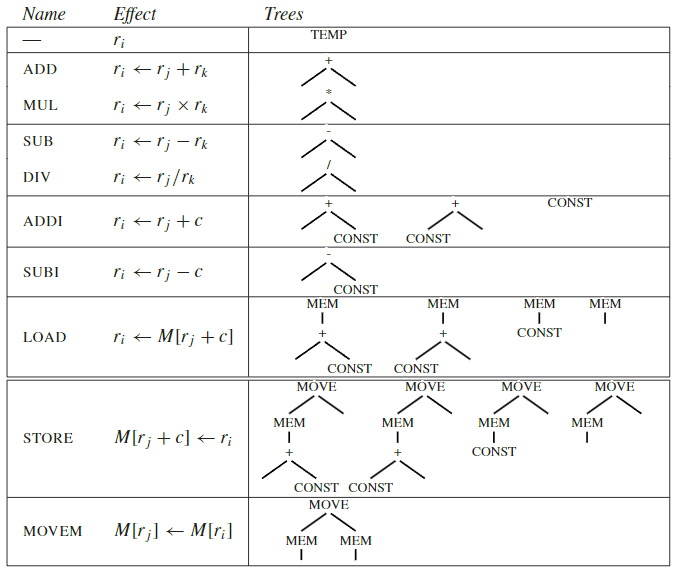
\includegraphics[width=0.42\textwidth]{pic/CP9/Jouette architecture}
    \caption{Jouette architecture}
    \label{fig:Jouette}
\end{figure}

一棵树可以有多种覆盖方式.
\begin{figure}[!htb]
    \centering
    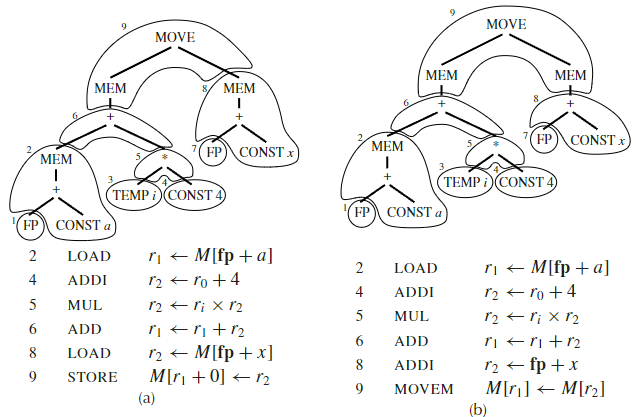
\includegraphics[width=0.309\textwidth]{pic/CP9/A tree tiled in two ways}
    \caption{A tree tiled in two ways}
\end{figure}

\subsubsection{Optimal and Optimum Tilings}
\begin{itemize}
    \item optimum tiling (最优覆盖): 覆盖的代价和是最小的覆盖,全局最优.
    \item optimal tiling (最佳覆盖): 不存在两个相邻的覆盖能连接成一个代价更小的覆盖,局部最优.
\end{itemize}
全局最优属于局部最优.


\subsection{Algorithm for Instruction Selection}
\subsubsection{Maximal Munch}
最佳覆盖的算法.

从树的根节点开始寻找 适 合 他 的 最 大 覆盖 (覆盖的节点数最多, 如果相等的可以任意选择其一), 按 照 Jouette 体系结构可能会覆盖其他几个节点; 对遗留的其他 子 树 也 进 行 相 同 操 作.

Maximal Munch 算 法 的 tiling 是从顶向下的,但是指令的生成是逆序的(很好理解,因为上层的覆盖指令需要下层的指令提供操作数,所以是逆序).


\subsubsection{Dynamic Programming}
可以找到最优覆 盖 , 子 问 题 是 子 树 的 覆 盖, 自下而上工作.

会给每个节点计算一个代价, 表示可以覆盖该节点为根的子树的指令序列最优的代价之和. 

对于一个节点 $n$, 先找到其所有子树的代价 $c_i$, 然后枚举节点 $n$ 所有可能的覆盖, 计算每种覆盖的代价 $c+\sum c_i$, 最后选择代价最小的覆盖.

不同的覆盖代价不同, 具体的代价书中没有给出, 看着默认都是 1, 即目标是覆盖的数量最少.


\subsubsection{Tree Grammar(树文法)}
DP 的推广. 使用 brain-damaged Jouette 体系.

\begin{figure}[!htb]
    \centering
    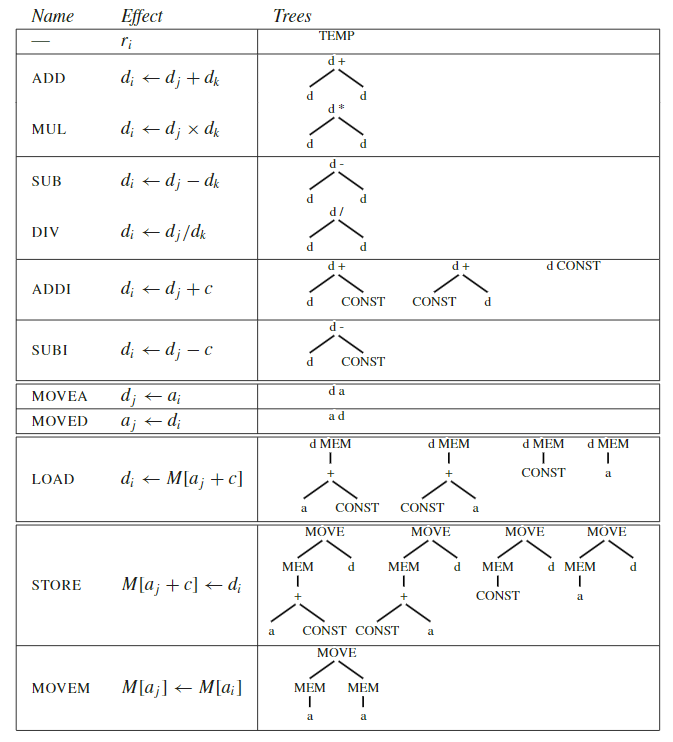
\includegraphics[width=0.42\textwidth]{pic/CP9/The Schizo-Jouette architecture}
    \caption{The Schizo-Jouette architecture}
\end{figure}

使用 CFG 来描述覆盖,文法具有高 度歧义性, 但是 DP 可以很好 处理给出最优的覆盖.

有两类寄存器:
\begin{itemize}
    \item a 寄存器:存地址;
    \item d 寄存器:存数据
\end{itemize}

\begin{figure}[!htb]
    \centering
    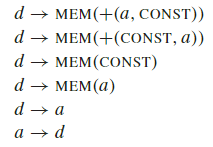
\includegraphics[width=0.22\textwidth]{pic/CP9/The grammar rules}
    \caption{The grammar rules for the LOAD , MOVEA and MOVED instructions}
\end{figure}


\subsubsection{Fast Match}
使用 switch-case 来匹配非叶子节点的 label.


\subsubsection{Efficiency of Tiling Algorithms}
$T$ 个覆盖,平均每个匹配的覆盖有 $K$ 个非叶子节点. $K'$ 是在给定子树中为确定匹配那个覆盖需要检查的最大节点个数(近似于最大覆盖的大小). 假定平均每个树节点可以与 $T'$ 个覆盖匹配. 输入树的节点为 $N$.
\begin{itemize}
    \item Maximal Munch: 平均只需要遍历 $N/K$ 个节点, 就可以覆盖整棵树, 所以 复杂度为 $O((K'+T')N/K)$
    \item DP: 需要遍历所有节点的所有覆盖可能, 复杂度为 $O((K'+T')N)$
\end{itemize}
DP 的其他常数也比 Maximal 大, 因为要遍历两遍. $K',K,T$ 是常数, 线性复杂度.


\subsection{CISC Machines}

RISC 机器特征:
\begin{enumerate}
    \item 32 个寄存器
    \item 仅有一类整数/指针寄存器
    \item 算数运算仅对寄存器进行操作
    \item 采用``三地址''指令$(r_1\leftarrow r_1+r_2)$
    \item 取指令和村指令只有 M[reg+const]模式
    \item 每条指令长度固定为32 位
    \item 每一条指令产生一个结果或作用,无副作用
\end{enumerate}

CISC 机器特征:
\begin{enumerate}
    \item 不多的几个寄存器(16,8,6)
    \item 寄存器分不同类型,某些操作只能在特定种类的寄存器上进行
    \item 算术运算可以通过不同的寻址模式访问寄存器和储存器
    \item 指令是``两地址''指令
    \item 有不同的寻址模式
    \item 有由变长操作码加变长寻址模式形成的变长指令
    \item 指令具有副作用(自增寻址方式)
\end{enumerate}

CISC 机器的特点解决难题:
\begin{enumerate}
    \item  寄 存 器 较 少 : 不 限 制 生 成TEMP 节点,假设寄存器分配能完成分配工作
    \item 寄存器分类:将操作数显示地传送到相应的寄存器中
    \item 两地址指令:增加一条额外的传送指令
    \item 算数运算可以访问存储器:指令选择阶段将每一个 TEMP 节点转化成一个寄存器引用.
    \item 若干种寻址模式:优点(破坏寄存器少;指令代码短)
    \item 变长指令:不管;
    \item 副作用指令
\end{enumerate}

三种解决办法:
\begin{enumerate}
    \item 忽略地址自增指令,希望其自动消失
    \item 在采取树型匹配的代码生成器的上下文中使用特别方式匹配特殊的习惯用法
    \item 使用完全不同的指令算法,基于 DAG 样式.
\end{enumerate}
    \newpage
\section{Liveness(活跃性) Analysis}
\subsection{Definition}
% \begin{definition}
%     A variable is \textbf{live} if it holds a value that may be needed in the future.
% \end{definition}
编译器需要分析程序的中间表示,以确定那些临时变量在同时被使用.如果一个变量的值在将来还需要使用,则变量是活跃的 (live),这种分析叫做活跃分析.

控制流图(control flow graph): 程序的每条语句都是流图的节点.


\begin{figure}[!htb]
    \centering
    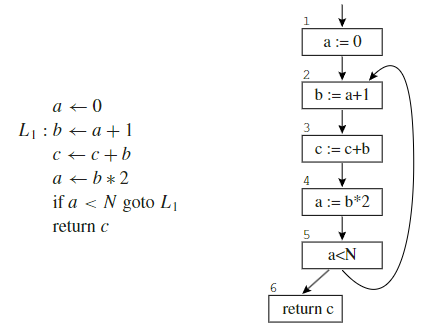
\includegraphics[width=0.309\textwidth]{pic/CP10/Control-flow graph of a program}
    \caption{Control-flow graph of a program}
\end{figure}


活跃范围(Liveness): 变量位索引的集合,变量在那几条边上活跃的边集合.

\begin{figure}[!htb]
    \centering
    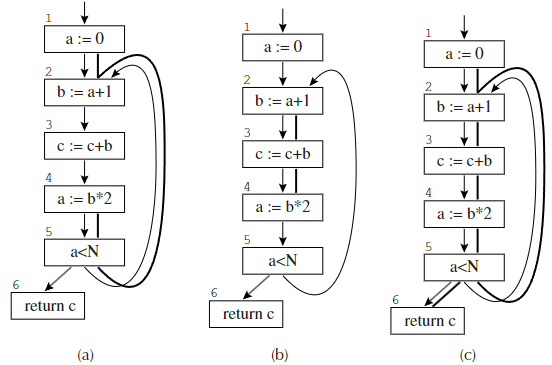
\includegraphics[width=0.42\textwidth]{pic/CP10/Liveness of variables}
    \caption{Liveness of variables $a, b, c$.}
\end{figure}

\subsection{Solution of Dataflow Equations}

\begin{itemize}
    \item 出边(out-edge):节点引向后继节点的边; 
    \item 入 边 (in-edge): 由 前 继 节 点 指 向 的边.
\end{itemize}
$succ[n]$ 是节点 $n$ 的后继节点; $pred[n]$ 是节点 $n$ 的前驱节点


\begin{itemize}
    \item 定义(define): 对变量和临时变量的赋值称为变量的定义;
    \item 使用(use): 使用出现在赋值号右边的变量.
\end{itemize}

活跃性(Liveness): 变量在边上活跃是指存在一条边通向一个使用该变量的有向路径,且不经过该变量的任何定义.
\begin{itemize}
    \item 如果变量在一个节点的所有入边上全是活跃的,那么该变量是入口 活 跃 的 (live-in); 
    \item 若 一个变量在一个节点的所有出边上都是活跃的,那么该变量在 该 节 点 是 出 口 活 跃 的(live-out).
\end{itemize}

\subsubsection{Calculation of Liveness}
就是计算流图每一个节点的 $in$ 和 $out$ 集合
\begin{equation}
    \begin{split}
        in[n]&=use[n]\cup (out[n]-def[n])\\
        out[n]&=\bigcup_{s\in succ[n]}in[s]
    \end{split}\label{eq:liveness}
\end{equation}

活跃性计算的迭代方法
\begin{algorithm}[H]
    \caption{Computation of liveness by iteration}
    \label{algo:liveness}
    \begin{algorithmic}
        \For{each $n$}
            \State $in[n]\leftarrow \{\};\ out[n]\leftarrow \{\}$
        \EndFor
        \Repeat
            \For{each $n$}
                \State $in'[n]\leftarrow in[n];\ out'[n]\leftarrow out[n]$
                \State $in[n]\leftarrow use[n] \cup (out[n] - def[n])$
                \State $\displaystyle out[n]\leftarrow \bigcup_{s\in succ[n]}in[s]$
            \EndFor
        \Until{$in'[n]=in[n]$ and $out'[n]=out[n]$ for all $n$}
    \end{algorithmic}
\end{algorithm}

\begin{figure}[!htb]
    \centering
    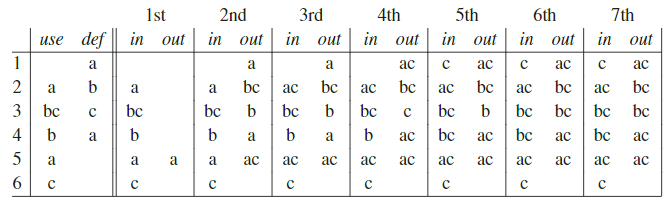
\includegraphics[height=0.14\textwidth]{pic/CP10/Liveness calculation following forward control-flow edges.}
    \caption{Liveness calculation following forward control-flow edges.}
\end{figure}

\begin{figure}[!htb]
    \centering
    \includegraphics[height=0.14\textwidth]{pic/CP10/Liveness calculation following reverse control-flow edges}
    \caption{Liveness calculation following reverse control-flow edges.}
\end{figure}

适当排序可以显著加快算法的收敛过程,一般要从程序末尾往前算,先算 $out$ 再算 $in$,可以显著提高速度和正确率. 信息活跃性是沿控制流箭头的反方向流动的,计算顺序同理.


时间复杂度: 
\begin{itemize}
    \item for 循环初始化 节 点 $in,out$ 需 要 $O(N^2)$; 
    \item repeat 循环 的时 间复杂度是 $O(N^4)$.
\end{itemize}
由于活跃信息大部分稀疏,实际运行时间在 $O(N)$ 和 $O(N^2)$ 之间.

\subsubsection{Representation of Sets}
\begin{itemize}
    \item 位数组(bit array): 程序中有 $N$ 个变量,用 $N$ 位二进制数表示集合
    \subitem 求并集对位数组求按位或
    \subitem 时间效率:对每个字有 $K$ 位的计算机, 并运算需要 $N/K$ 次操作
    \item 有序变量表:链表的成员是组成集合的元素
    \subitem 并集通过合并链表实现
    \subitem 时间开销和求并集的集合大小成线性.
\end{itemize}

集合稀疏(平均少于 $N/K$)用有序链表表示速度会更快(越稀疏越快); 集合密集位数组表示更好.

\subsubsection{Least Fixed Points}
\textbf{Equation} \ref{eq:liveness} 的解只是保守的近似解,只能保证生成的代码是正确的, 但是所使用的寄存器可能比实际需要的多. 

\begin{theorem}
    \textbf{Equation} \ref{eq:liveness} 有一个以上的解.
\end{theorem}
\begin{proof}
    增加更多的变量后, 结果仍是 \textbf{Equation} \ref{eq:liveness} 的解.
\end{proof}

\begin{theorem}
    \textbf{Equation} \ref{eq:liveness} 的所有解都包含最小解(least solution). 
\end{theorem}

\textbf{Algorithm} \ref{algo:liveness} 所计算的就是最小解. 

\subsubsection{Static v.s. Dynamic Liveness}
\begin{theorem}[Halting Problem]
    不存在程序 $H$, 其以任意程序 $P$ 和 输入 $X$ 作为自己的输入. 当 $P(X)$ 停止时返回真, 否则返回假. 
\end{theorem}

\begin{corollary}
    不存在程序 $H'(X, L)$, 对任何程序 $X$ 和其中标记 $L$, 可以判断 $X$ 在执行中是否到达过 $L$.
\end{corollary}
意思是不存在一个通用程序能算出每一个标记是否达到. 


动态判断及其静态的近似:
\begin{itemize}
    \item 动态活跃(Dynamic liveness): 如果程序从节点 $n$ 执行到 使用 $a$ 之间没有经过 $a$ 的任何 定义,那么变量 $a$ 在节点 $n$ 是动态活跃的.
    \item 静态活跃(Static liveness): 如果存在着一条从 $n$ 到 使用 $a$ 的控制流路径,且此路径上没有 $a$ 的任何 定义,那么变量 $a$ 在节点 $n$ 静态活跃的.
\end{itemize}

\subsubsection{Interference Graphs}
\begin{definition}
    两个临时变量不能分配到同一个寄存器的情况称为冲突(interference).
\end{definition}

冲突原因:
\begin{enumerate}
    \item 临时变量在程序的同一点同时活跃
    \item 某些寄存器必须被使用时,临时变量不能占用这些寄存器.
\end{enumerate}

\begin{figure}[!htb]
    \centering
    \begin{subfigure}{0.12\textwidth}
        \centering
        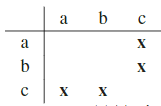
\includegraphics[width=\textwidth]{pic/CP10/Matrix.png}
        \caption{Matrix}
    \end{subfigure}
    \begin{subfigure}{0.08\textwidth}
        \centering
        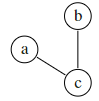
\includegraphics[width=\textwidth]{pic/CP10/Graph.png}
        \caption{Graph}
    \end{subfigure}
    \caption{Representations of interference}
\end{figure}

绘制冲突图的办法:为新定义 (def) 添 加 冲 突 边, 即
\begin{enumerate}
    \item 对 变 量 $a$ 非 MOVE 指令的定义 , 以及在该指令节 点 $n$ 处,任意 $b_i\in out[n]$,添 加 冲 突 边 $(a,b_i)$
    \item 对 于 节 点标号为 $n$ 的 MOVE 指令 $a\leftarrow c$,对 $b_i\in out[n]$ 且 $b_i\ne c$, 添加边 $(a,b_i)$. 
    \subitem 注:可以给 $(a,c)$ 画上虚线,便于寄存器 分配的 coalesce.
\end{enumerate}



    \newpage
\section{Register Allocation}
通过染色算法对冲突图求解.
\subsection{Coloring by Simplification}
寄存器分配与图染色都是 NP-complete 问题. 这里使用一种线性近似算法, 分为构建, 简化, 溢出, 选择四个阶段. 

\begin{enumerate}
    \item 构建: 构建冲突图.
    \item 简化: 启发式图染色. 将图中度数 $<K$ (寄存器个数) 的节点删除, 并压入一个栈中. 直到剩下节点度数都 $\ge K$, 无法继续简化. 
    \item 溢出: 称目前剩下为高度数(significant degree, 度$\ge K$)点. 选择与剩下其他节点无冲突的, 代表临时变量的点作为溢出, 将其删除并标记为潜在溢出(potential spill)压入栈中. 然后继续简化. 
    \item 选择: 从空图开始, 将点从栈中弹出, 加入到图中并染色.  每次加入节点, 其必须被染色. 
    \subitem 若为潜在溢出的点, 其可能无法被染色, 则将其标记为实际溢出(actual spill), 然后不管其继续弹出节点. 
    \subitem 但潜在溢出的点也可能被成功染色(其周围有节点颜色相同), 此时称为乐观染色(optimistic coloring).
    \item 重开: 对实际溢出的节点, 重写程序通过读写内存对其进行操作. 但就算如此, 读写也需要额外几个临时寄存器, 此时对于重写的程序, 重新构建冲突图, 跑染色算法. 多次迭代直到简化阶段不会溢出, 一般而言, 一两次迭代即可. 
\end{enumerate}

假设 $a$ 发生了实际溢出, 则 $a$ 必须通过读写内存对其进行操作. 对其 def 与 use 的修改如下:
\begin{enumerate}
    \item 对于 $a$ 的每个 use, 新建 $a_i$, 从 $M[a_{loc}]$ 读取 $a$. 
    \subitem $c\leftarrow a \Rightarrow a_1\leftarrow M[a_{loc}], c\leftarrow a_1$
    \item 对于 $a$ 的每个 def, 新建 $a_i$, 通过其写入 $M[a_{loc}]$.
    \subitem $a\leftarrow c \Rightarrow a_2\leftarrow c, M[a_{loc}]\leftarrow a_2$
\end{enumerate}

\begin{example}
    假设有四个寄存器. 

    \begin{figure}[!htb]
        \centering
        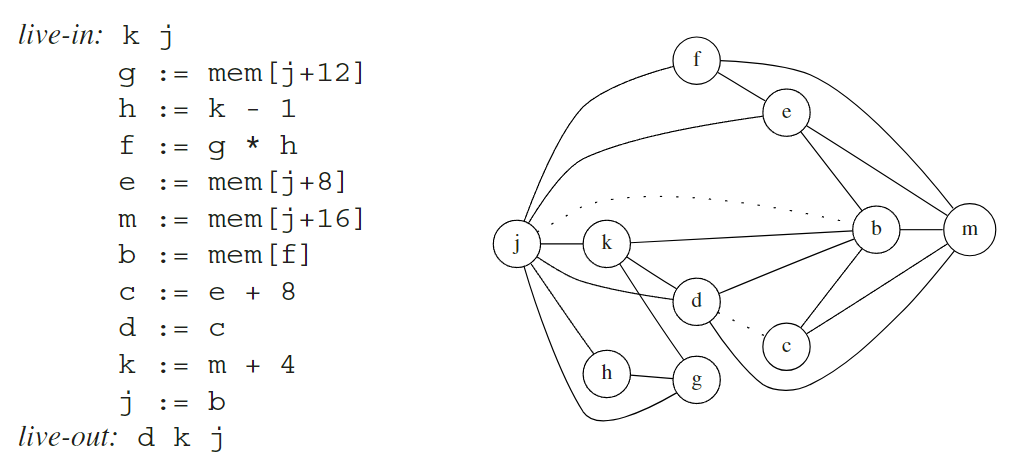
\includegraphics[width=0.42\textwidth]{pic/CP11/Interference graph for a program}
        \caption{Interference graph for a program}
        \label{fig:Interference-graph}
    \end{figure}
    
    \textbf{Figure} \ref{fig:Interference-graph} 简化就可以删除全部节点了. 然后依次弹出并染色. 

    \begin{figure}[!htb]
        \centering
        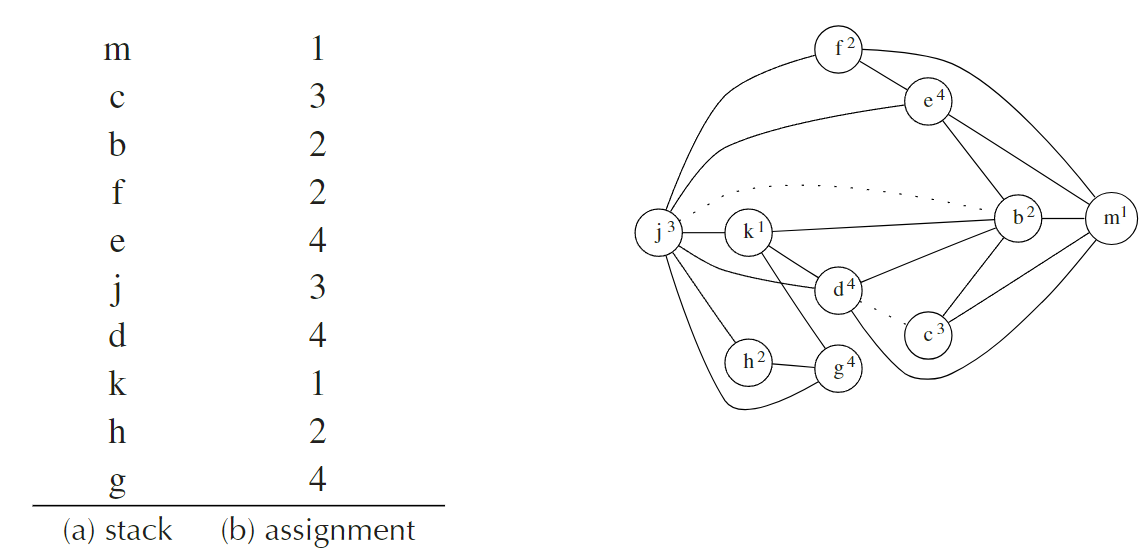
\includegraphics[width=0.42\textwidth]{pic/CP11/Simplification stack, and a possible coloring}
        \caption{Simplification stack, and a possible coloring}
    \end{figure}
    
    
\end{example}

\subsection{Coalescing}
删除冗余的 MOVE 指令. 若 MOVE 的 src 与 dst 之间不冲突, 则将其合并为新节点, 与新节点冲突的点是二者的并集. 理论上, 任意一对不冲突的点都可以被合并. 但合并可能导致原本可被染色图不能被染色. 

所以引出安全的合并策略:
\begin{enumerate}
    \item Briggs: 如果 $a,b$ 合并后的节点 $ab$ 的高度数邻居个数 $<K$,则 $a, b$ 可以合并.
    \item George: 对于 $a$ 的每个邻居 $t$, 若 $t$ 与 $b$ 冲突, 或者 $t$ 是低度数点(度$<K$), 则 $a,b$ 可以合并. 
\end{enumerate}

这 两 种 策 略 都 是 保 守 的(conservative), 因 为其合并不会改变图的着色性. 策略执行后可能仍有多余的 MOVE 指令, 但这至少比溢出好.


\begin{figure}[!htb]
    \centering
    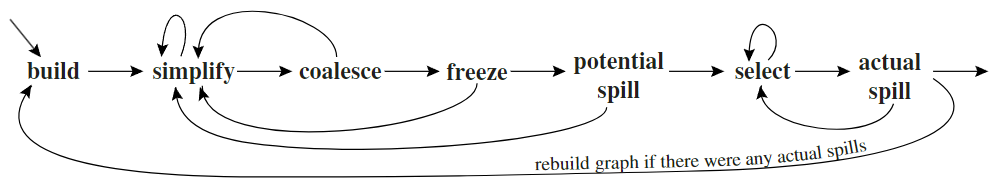
\includegraphics[width=0.42\textwidth]{pic/CP11/Graph coloring with coalescing}
    \caption{Graph coloring with coalescing}
\end{figure}

带合并的图染色算法:
\begin{enumerate}
    \item 构建: 构建冲突图, 将节点分类为 move-related 与 non-move-related. move-related 节点指此点是 MOVE 的 src 或 dst. 
    \item 简化: 删除低度数($<K$) 的 non-move-related 节点, 并压入栈中. 直到无法简化. 
    \item 合并: 运行保守的合并策略, 每次合并两个节点(删除相关 MOVE 指令), 若结果是 non-move-related, 则继续简化. 重复简化合并直到剩下的都是高度数或 move-related 节点. 
    \item 冻结: 寻找一个度数较低的 move-related 节点, 放弃对其相关 MOVE 指令的合并, 将此 MOVE 指令相关的点标记为 non-move-related. 然后继续简化合并.
    \item 溢出: 若没有低度数节点, 选择高度数节点作为潜在溢出并删除压入栈中. 
    \item 选择:将点从栈中弹出, 加入到图中并染色. 
\end{enumerate}

\begin{example}
    仍是四个寄存器, 以 \textbf{Figure} \ref{fig:Interference-graph} 为例. 

    只有 $b,c,d,j$ 四个点是 move-related 的. 简化 $g,h,k$. 然后合并 $cd, bj$. 最后完成所有的简化. 不需要溢出. 

    \begin{figure}[!htb]
        \centering
        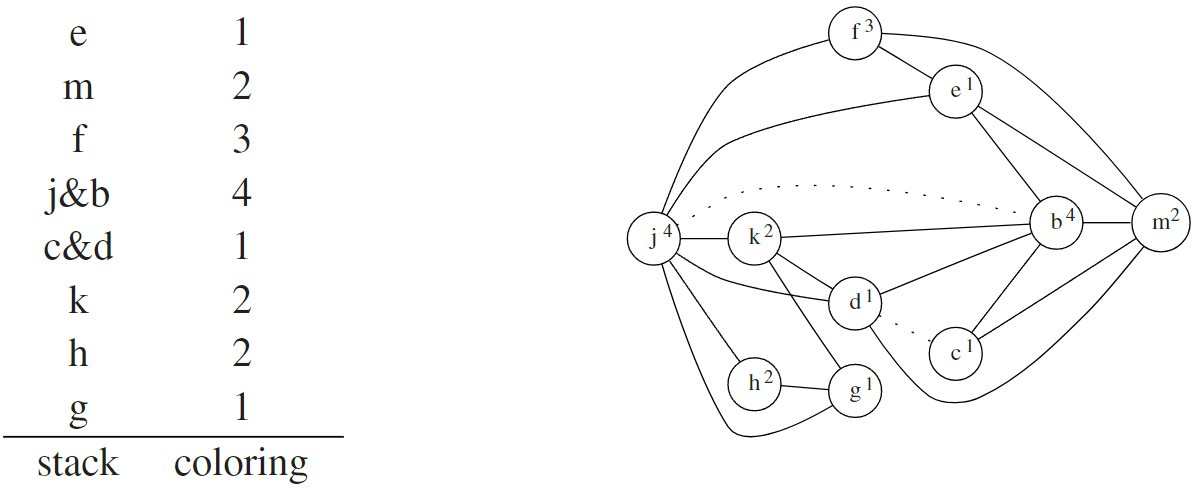
\includegraphics[width=0.42\textwidth]{pic/CP11/A coloring, with coalescing}
        \caption{A coloring, with coalescing}
    \end{figure}
    
\end{example} 

若冲突图中两个节点既有虚线又有实现, 则称之为受约束的(constrained). 对此不将其考虑为 move-related. 

\subsection{Precolored Nodes}
有一些临时变量是预着色的, 代表的是机器寄存器, 参数寄存器, 帧指针, 返回值寄存器等. 预着色的点必须相互冲突, 一般来说, 一个颜色只会对一个节点预着色. 

选择与合并操作可以给一个普通点被预着色的颜色, 只要没有冲突. 特别的, 当一个预着色节点与普通节点使用 George 合并时, 需要将普通节点作为 $a$, 检查普通节点的邻居是否满足合并条件. 

预着色节点特性:
\begin{enumerate}
    \item 无法简化
    \item 无法溢出(认为此点的度无限大)
    \item 可以参与合并.
\end{enumerate}

染色算法通过简化合并溢出来工作, 直到只剩下预着色节点, 然后才能开始向冲突图中加入其他节点. 预着色节点不能溢出所以前端必须使他们的活跃范围保持较小, 可以通过 MOVE 指令来实现. 

对于节点 $a$, 其溢出优先级计算公式: 
\begin{align*}
    Priority = \frac{Out_{use+def}+10\times In_{use+def}}{D}
\end{align*}
其中,
\begin{itemize}
    \item $Out_{use+def}$ 为 $a$ 在循环外的 use 与 def 总数.
    \item $In_{use+def}$ 为 $a$ 在循环内的 use 与 def 总数.
    \item $D$ 为 $a$ 的度, 只包含实线. 
\end{itemize}

优先级值越小, 说明优先级越高. 表示优先溢出不被经常使用的高度数节点. 

% \subsection{Graph Coloring Implementation} 这章讲如何具体实现算法, 考试不太可能考, 跳了.

% \subsection{Register Allocation for Trees} 也是讲代码, 跳了
    \newpage
\section{Garbage Collection}

\begin{definition}[Garbage]
    Heap-allocated records that are not reachable by any chain of pointers from program variables are garbage.
\end{definition}


不存在一个通用程序能算出每一个变量是否活跃, 所以使用一个保守的近似: 要求编译器保证所有活跃记录是可达的(reachable), 并最小化可达的不活跃记录. 

\subsection{Mark-and-sweep Collection}
程序变量与堆分配记录可以构成一张有向图. 变量就是图的一系列根.

\begin{definition}[reachable]
    A node $n$ is reachable if there is a path of directed edges $r \to\cdots \to  n$ starting at some root $r$.
\end{definition}

算法原理:
\begin{enumerate}
    \item 标记: 使用 DFS 标记所有可达节点
    \item 清扫: 未被标记的节点都是垃圾, 从头到尾扫描堆内存, 将未标记的节点加到空闲表(freelist)中, 同时清除已标记节点的标记. 
\end{enumerate}

% \begin{algorithm}[H]
%     \caption{Mark-and-sweep Collection}
%     \begin{algorithmic}
%         \Function{Dfs}{$x$}
%             \If{ $x$ 是堆中的指针}
%                 \If{记录 $x$ 没有被标记}
%                     \State 标记 $x$
%                     \For{记录 $x$ 的每个域 $f_i$}
%                         \State DFS($x, f_i$)
%                     \EndFor
%                 \EndIf
%             \EndIf
%         \EndFunction
%         \State Mark phase:
%         \For{每个根 $v$}
%             \State DFS($v$)
%         \EndFor
%         \State Sweeo phase:
%         \State $p$ $\leftarrow$ 堆的首地址
%         \While{$p<$ 堆的尾地址}
%             \If{记录 $p$ 被标记}
%                 \State 清除 $p$ 标记
%             \Else
%                 \State 让 $f_1$ 为 $p$ 的第一个域
%                 \State $p.f_1 \leftarrow $ 空闲表
%                 \State 空闲表 $\leftarrow p$ 
%             \EndIf
%             \State $p\leftarrow p+$(记录 $p$ 的大小)
%         \EndWhile
%     \end{algorithmic}
% \end{algorithm}

\subsubsection{Cost of garbage collection}
假设大小为 $H$ 个字的堆中, 有 $R$ 个字可达, 则一次垃圾回收的代价是 $c_1R+c_2H$, 其中 $c_1, c_2$ 为常数. 

最终每个垃圾的均摊回收代价是 
\begin{align*}
    \frac{c_1R+c_2H}{H-R}
\end{align*}
若 $\frac{R}{H}>0.5$, 回收器应该向 OS 申请更大的内存, 以增大 $H$.

\subsubsection{Optimization}
对算法的空间与时间常数进行优化. 

\begin{itemize}
    \item Using an explicit stack: 将 DFS 的递归改写为循环. 因为递归的 DFS 其运行时的栈可能超过总的堆大小, 所以用显式的栈代替使用堆.
    \item Pointer reversal: 压栈时使用 $x.f_i$ 指向其父节点, 弹栈时再恢复 $x.f_i$ 原本的值, 这样连显示的栈都不需要. 只需要额外的 $done$ 数组作为 $x$ 子域的下标.
\end{itemize}

DFS 中, $x$ 是当前节点, $t$ 是父节点, $y$ 是子节点, $done[x]$ 用于索引 $x.f_{done[x]}$ 作为下一个子域. 

\begin{figure}[!htb]
    \centering
    \includegraphics[width=0.309\textwidth]{pic/CP13/Depth-first search}
    \caption{DFS}
\end{figure}


\subsubsection{An Array of Freelists} 
$freelists$ 使用空闲域的大小作为索引, 存储邻接链表, 方便之后使用. 比如想要大小为 $i$ 的域, 把 $freelists[i]$ 的头取出即可. 也可以取出 $freelists[j](j>i)$, 然后把剩下的空闲域插入 $freelists[j-i]$.


\subsubsection{Fragment}
\begin{itemize}
    \item 外部碎片(external fragmentation): 想分配一个 $n$ 大小的空间, 但是空闲空间均小于 $n$.
    \item 内部碎片(internal fragmentation): 实际使用大小为 $n$ , 却分 配 了 大 小 为 $K(K>n)$ 的 空 间, 未使用的空间在记录内而不是在空闲表中.
\end{itemize}


\subsection{Reference Counts}
算法原理: 记住每个记录有多少指针指向其, 计数和每个记录储存在一起. 

\begin{itemize}
    \item 当 $p$ 写入 $x.f_i$ 时, $p$ 的引用数要增加, $x.f_i$ 之前内容的引用数要减少. 
    \item 若 $r$ 的引用数为 0, 将 $r$ 加入到 $freelist$ 中, 并减少 $r$ 指向的其他记录的引用数. 
\end{itemize}

有一个改进是在将 $r$ 从 $freelist$ 中删除时,再递归地减少 $r.f_i$ 的计数:
\begin{enumerate}
    \item 能将递归减少的动作分解为较短的操作, 使程序的运行更加平滑(对对交互式程序或实时程序好)
    \item 递归减少动作只需要在分配 $r$ 时进行. 
\end{enumerate}

但有两个大问题:
\begin{enumerate}
    \item 无法回收成环的垃圾.
    \item 增加引用计数所需的操作代价很大.
\end{enumerate}

解决``环''的办法:
\begin{enumerate}
    \item 让程序员手动断开所有循环引用, 这比手动管理内存要简单, 但也并不优雅.
    \item 将标记清理(快速, 无中断地回收)和引用计数(回收环)相结合.
\end{enumerate}

引用计数的缺点大于优点, 所以极少使用. 

\subsection{Copying Collection}
\begin{enumerate}
    \item 将堆分为两块区 域 from-space 和 to-space; 当 前 的 内 存 放 到 from-space 中 
    \item 在 to-space 构造一个同构的副本, 副本空间利用上更紧凑: 占据连续的不含碎片的储存单元
    \item from-space 和 to-space 互换, 然后抛弃 from-space. 
\end{enumerate}


\begin{figure}[!htb]
    \centering
    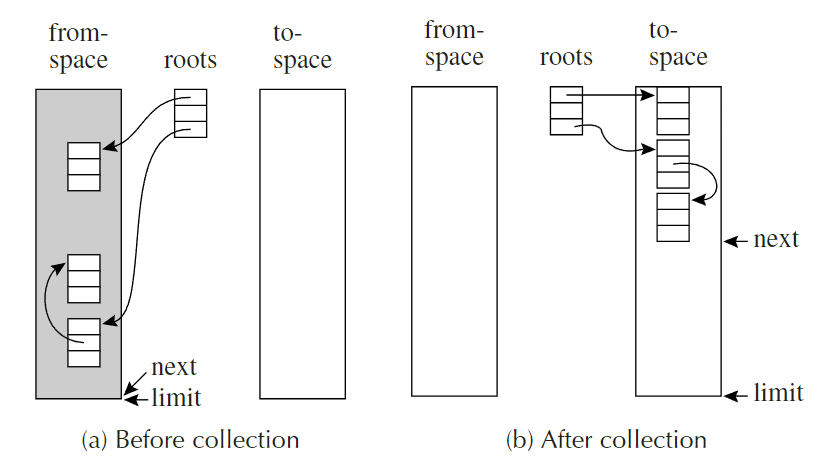
\includegraphics[width=0.42\textwidth]{pic/CP13/Copying collection}
    \caption{Copying collection}
\end{figure}

算法流程:
\begin{enumerate}
    \item 回收初始化: 初始化指针 next 指向 to-space 的开始. 每当 from-space 发现一个可达记录, 便把它复制到 to-space 的 next 所指位置, 同时使 next 增 加 该 记 录 的 大 小. 
    \item 转递(forwarding): 使一个指向 from-space 的指针 $p$ 转而指向 to-space. 有三种情况:
    \begin{enumerate}
        \item 若 $p$ 指向的 from-space 已经被复制, 则 $p.f_1$ 是一个特殊的转递指针(forwarding pointer)指向了副本所在. 因为只有这种指针指向了 to-space, 可以很容易地分辨. 
        \item 若 $p$ 指向的 from-space 未被复制, 则将其复制到 next 所在位置, 然后将 $p.f_1$ 变为转递指针. 因为其已经被复制了, 所以可以覆写 $f_1$.
        \item 若 $p$ 不是指针或指向了 from-space 之外, 不做任何事. 
    \end{enumerate}
\end{enumerate}

\subsubsection{Cheney's algorithm}
使用 BFS 遍历可达数据. 

\begin{itemize}
    \item 在 to-space 上, 位于 scan 与 next 之间包含了已经被复制到 to-sapce, 但是其子域还没有转递的记录, 他们的子域仍指向着 from-space. 
    \item 在 scan 之前包含了被复制且被转递的记录, 其中所有指针都指向 to-space.
\end{itemize}

但其空间局部性不好, 比如说 $a+8$ 指向的地址就不是 $a[8]$, 因为 BFS 会把 $a[8]$ 放到诸如 $b[\ ],c[\ ]$后面.  DFS 的局部性很好, 但需要各种复杂的常数优化. 所以结合 BFS 与 DFS, 用 BFS 寻找需要复制的记录, 复制时使用 DFS 复制. 

\subsubsection{Cost of garbage collection}
假设大小为 $H$ 个字的堆中, 有 $R$ 个字可达, 因为 $H$ 被分为了两部分, 所以只需要回收 $\frac{H}{2}-R$ 的垃圾. 对每个垃圾的均摊回收代价为
\begin{align*}
    \frac{c_3R}{\frac{H}{2}-R}
\end{align*}
其中 $c_3$ 是常数. 


\subsection{Interface to the Compiler}

\subsubsection{Fast Allocation}
使用复制回收(copying collection)的方式回收垃圾, 以便分配空间是一个连续的空闲区域. 区 域 的 末 端 是 limit, next 指向下一个空闲单元.

分配大小为 $N$ 的记录的步骤如下: 
\begin{enumerate}
    \item 调用分配函数
    \item 若 $next+N<limit$ 则继续, 否则调用垃圾回收.
    \item 将 $next$ 复制到 $result$
    \item 清理 $M[next], M[next+1],\dots,M[next+N-1]$
    \item $next\leftarrow next+N$
    \item 从分配函数返回. 
    \begin{enumerate}
        \item 将 $result$ 赋值到计算上有用的地方.
        \item 将要 用 到 的 值 储 存 到 该 记 录 
    \end{enumerate}
\end{enumerate}

使用内联展开(inline expanding, 将函数调用替换为函数本体)可以省略 1) 和 6); 与 a. 结合可以消除 3); b. 也可以消除 4); 2), 5) 不能被消除. 但若是多个分配可以被合并优化. 至此, 分配就减少到了4条指令. 


\subsubsection{Describing Data Layouts}
垃圾回收器需要对任意数据类型进行操作, 所以需要确定每条记录的子域类型及数量. 简单的方法是用每个对象指针的第一个字指向一个描述记录(descripter record), 其包含对象总大小, 以及每个域指针的位置. 

垃圾回收器需要知道哪些内存地址是指针, 才能正确地跟踪对象间的引用关系, 避免错误地回收正在使用的对象. 所以编译器需要生成指针映射(pointer map)来描述程序运行过程中每个时刻哪些位置存储着指针. 

具体步骤:
\begin{enumerate}
    \item 识别指针: 编译器需要识别出所有可能包含指针的变量, 包括堆记录, 临时变量和局部变量, 无论它们存储在寄存器还是活动记录(activation record)中. 
    \item 指针映射的时机: 由于活跃指针的集合在每条指令执行后都可能发生变化, 所以为每条指令都生成指针映射是不现实的. 因此, 编译器只在垃圾回收可能开始的点生成指针映射, 这些点包括:
    \begin{itemize}
        \item 调用 alloc 函数的地方, 因为分配新内存可能会触发垃圾回收. 
        \item 每个函数调用的地方, 因为被调用的函数可能直接或间接地调用 alloc 函数. 
    \end{itemize}
    \item 指针映射的组织: 指针映射使用函数返回地址作为键, 因为返回地址是垃圾回收器在下一个活动记录中看到的内容. 每个返回地址对应一个活跃指针集合, 描述了在该返回地址处哪些寄存器或栈帧位置存储着指针. 
    \item 垃圾回收过程: 垃圾回收器从栈顶开始向下扫描, 逐帧查找活跃指针. 
    \begin{itemize}
        \item 每个返回地址都指向一个指针映射条目, 该条目描述了下一帧的信息. 
        \item 在每一帧中, 垃圾回收器根据指针映射标记/转递(取决于垃圾回收方式)该帧中的所有活跃指针. 
    \end{itemize}
    \item callee-save 寄存器: 对于 callee-save 寄存器, 需要特殊处理. 
    \subitem 例如, 函数 $f$ 调用 $g$, $g$ 调用 $h$. 函数 $h$ 知道它将一些 callee-save 寄存器保存在其栈帧中, 并在其指针映射中记录了这一事实, 但 $h$ 不知道哪些寄存器是指针. 因此, $g$ 的指针映射必须描述在调用 $h$ 时, 哪些 callee-save 寄存器包含指针, 哪些是从 $f$ “继承”下来的.
\end{enumerate}


\subsubsection{Derived Pointers}
派生指针是指那些不直接指向堆记录起始地址的指针, 它们可能指向记录的中间、之前或之后. 


比如说, 考虑表达式 $a[i-2000]$, 它可以被编译器优化为: 
\begin{align*}
    t_1 &\leftarrow a - 2000\\
    t_2 &\leftarrow t_1 + i \\
    t_3 &\leftarrow M[t_2]
\end{align*}
其中, $a$ 是一个指向数组的指针, $t_1$ 就是一个派生指针, 它指向 $a$ 所指向数组的前 2000 个元素之前的位置. 

如果在循环中使用 $a[i-2000]$, 编译器可能会将 $t_1 \leftarrow a - 2000$ 提升到循环外, 以避免重复计算. 如果循环中还包含内存分配, 并且在 $t_1$ 仍然活跃时发生垃圾回收, 垃圾回收器可能会被 $t_1$ 这样的派生指针迷惑, 因为它不指向对象的起始地址, 甚至可能指向不相关的对象. 

为了解决这个问题, 编译器需要在指针映射中标识出每个派生指针, 并记录它所依赖的基指针(base pointer). 当垃圾回收器将基指针 $a$ 移动到新地址 $a'$ 时, 它需要根据基指针的移动量来调整派生指针 $t_1$ 的值, 即将 $t_1$ 更新为 $t_1 + a' - a$. 

由于派生指针依赖于基指针, 所以在编译器的活跃性分析中, 派生指针会隐式地保持其基指针的活跃状态. 也就是说, 只要派生指针还活跃, 它的基指针也必须被视为活跃的, 不能被回收.  % 1-3, 7
    % 只考小题, 抄了某个佬的笔记  https://cubicy.icu/compiler-construction-principles/#Part-19-%E9%9D%A2%E5%90%91%E5%AF%B9%E8%B1%A1-OOP
    \newpage
\section{Object-Oriented Languages} 
面向对象语言 = object-oriented language = OO language = class-based language
\begin{itemize}
    \item (几乎)所有值都是对象(object)
    \item 对象属于某个类, 或者说对象是某个类的实例(instance)
    \item 对象封装了状态(也就是成员变量 fields)与行为(也就是成员方法 methods)
\end{itemize}

重要概念:
\begin{itemize}
    \item 继承(inheritance): 派生类继承基类的特性
    \item 封装(encapsulation): 隐藏不该被外部接触到的接口
    \item 多态(polymorphism): 对象可以以不同形态呈现
\end{itemize}


\subsection{Classes}
拓展 Tiger 以支持对象. 不考大题, 就不详细记了. 


在 Tiger 中实现类需要解决如下问题:
\begin{itemize}
    \item Field layout: 某个类的各个 fields 在内存中如何放置、访问? 换句话说, 如何确定某个实例的 field 内存地址相对这个实例初始地址的偏移量? 
    \item Method dispatch: 调用某个实例的方法时, 如何找到正确的方法位于何地址? 是派生类的实现, 还是基类的实现, 还是基类的基类的实现 ? 
    \item Membership test: 如何检查给定实例是否是给定类的实例? 
\end{itemize}

\subsection{Single Inheritance of Data Fields}
单继承single-inheritance(SI): 每个类最多只能继承一个基类, 因此继承关系图是一棵树. 

\subsubsection{Field layout}
使用 *prefixing

\begin{figure}[!htb]
    \centering
    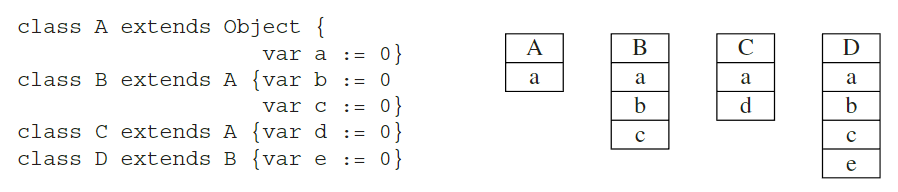
\includegraphics[width=0.42\textwidth]{pic/CP14/Single inheritance of data fields.}
    \caption{Single inheritance of data fields.}
\end{figure}


派生类新增的 fields 跟在基类的后面.  这使得我们可以正确处理多态: 例如把Cat当作Animal看待, 访问Animal的 fields 时相当于屏蔽了新增的 fields; 基类的各个 fields 偏移量不会因为这是个派生类实例发生变化, 仍然是已知的. 这避免了不安全的内存访问. 

\subsubsection{Method dispatch}
每个 method 编译成一段代码(称为 method instance), 编译方式和普通函数几乎无异. 比如 $A$ 中的 $f()$ 就编译为一段代码, 可用 $A_f$ 这样 label 标记函数地址. 机器码中, 函数起始地址使用一个LABEL标出. 

每个类都对应一个 class decriptor, 里面包含了描述这个类的一些必要信息: 
\begin{itemize}
    \item 一个指向基类的指针
    \item 一个列表, 包含这个类所有的 method instances
\end{itemize}

对于 static method 的调用 $x.f()$, 编译器将会: 
\begin{enumerate}
    \item 找到对象 $x$ 对应的类, 记为 $C$.
    \item 如果 $C$ 中有 $f$, 则直接得出 $x.f()$ 翻译结果为 $C_f$; 否则继续向上(在基类中)寻找. 
    \item 假设 $C$ 的基类为 $B$, 在 $B$ 中查找 $f$, 如找到则得出 $x.f()$ 翻译结果为 $B_f$; 否则继续向上(在基类中)寻找. 
    \item $\dots$
    \item 直到在某个祖先中找到为止(或是一路找到Object还没有则报错), 调用它. 
\end{enumerate}

对于 dynamic method 的处理略复杂:
\begin{itemize}
    \item 每个类维护一个 dispatch vector (例如 C++ 中的虚表 vtable = virtual table = VMT = virtual methods table) 储存每个 method 的地址. 
    \subitem 建立方式类似 prefixing: 派生类中新声明的方法跟在基类 dispatch vector 的后面; 不过如果有基类的 method 被重写了, 也要替换成自己重写后 method 的地址. 这样, 每个方法的偏移量是确定的. 
    \item 每个对象都关联某个 vtable: 对象的开头储存一个指针指向对应 class descriptor , 里面就有 vtable. 
    \item 需要动态查找(lookup), 有额外的开销. 
\end{itemize}

\begin{figure}[!htb]
    \centering
    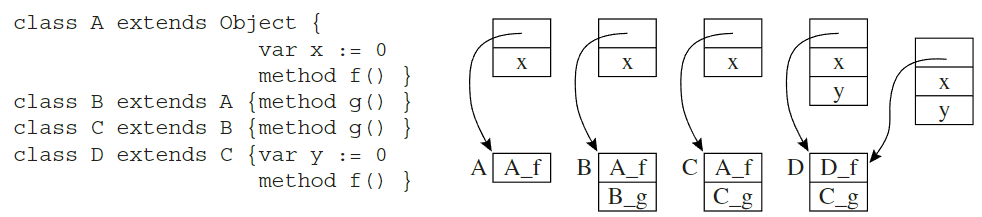
\includegraphics[width=0.42\textwidth]{pic/CP14/Class descriptors for dynamic method lookup}
    \caption{Class descriptors for dynamic method lookup}
\end{figure}

对于 dynamic method 的调用 $x.f()$, 编译器将会: 
\begin{enumerate}
    \item 在 $x$ 的 0 偏移处(开头)找到 class descriptor $d$.
    \item 由于方法 $f$ 的偏移量是确定的(记为 $F$), 从 $d$ 中 $F$ 偏移处获取 $f$ 的函数地址. 
    \item 调用f.
\end{enumerate}

\begin{figure}[!htb]
    \centering
    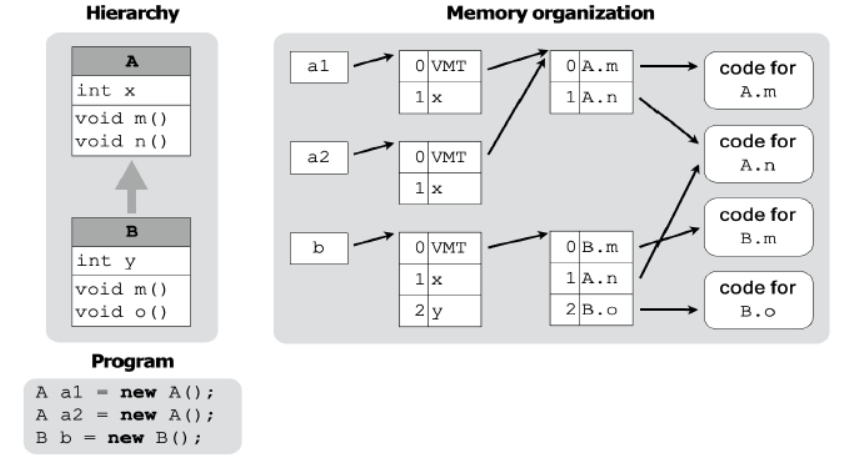
\includegraphics[width=0.309\textwidth]{pic/CP14/dynamic method}
    \caption{dynamic method}
\end{figure}


\subsection{Multiple Inheritance of Data Fields}
多继承multiple-inheritance(MI): 每个类可以继承多个基类, 因此继承关系图是有向无环图(DAG). % 我抄的佬认为多继承是纯纯的方向错误, C++为了多继承打了一堆补丁最后还是破破烂烂. 

\begin{figure}[!htb]
    \centering
    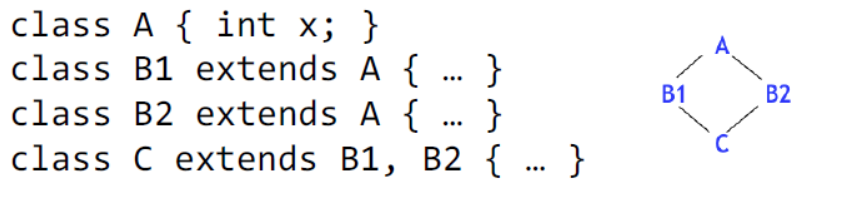
\includegraphics[width=0.309\textwidth]{pic/CP14/菱形继承}
    \caption{菱形继承}
\end{figure}


引入了经典的菱形继承问题: 
\begin{itemize}
    \item 歧义: 如果 $B1$ 和 $B2$ 中都有 method $m$, 那么 $C$ 的实例 $c$ 上调用 $c.m()$ 时应该调用哪个 $m$? 无法确定. 
    \item field replication: 对于 $A$ 中的一个 field $x$, 由于 $B1$ 和 $B2$ 中都继承了 $A.x$, 最终 $C$ 中会有重复的两个 $x$ 都来自 $A$.
\end{itemize}

\subsubsection{Field layout}
通过图染色获取. 

\begin{figure}[!htb]
    \centering
    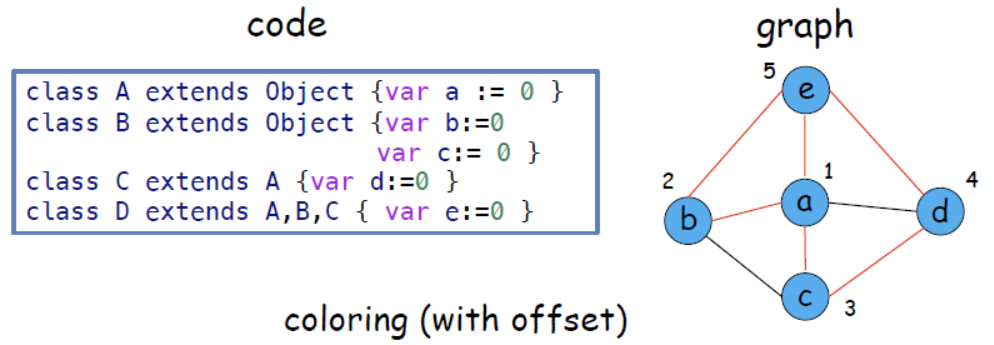
\includegraphics[width=0.42\textwidth]{pic/CP14/Multiple inheritance}
    \caption{Multiple inheritance}
    \label{fig:Multiple inheritance}
\end{figure}

目标: 静态分析所有类, 为每个 field 的找到一个固定偏移量. 如果不同 field 在同一个类中出现, 则不能共享同一个偏移量. 
\begin{itemize}
    \item 节点: 不同的 field 名
    \item 边: 同时在某个类中出现的 field 则连边
    \item 颜色: 最终偏移量(0, 1, 2, $\cdots$)
\end{itemize}

例如从 \textbf{Figure} \ref{fig:Multiple inheritance} 将得到 \textbf{Figure} \ref{fig:Multiple inheritance of data fields}.

\begin{figure}[!htb]
    \centering
    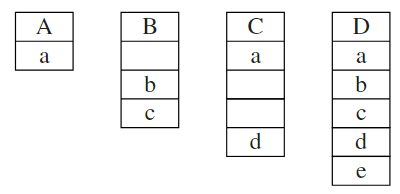
\includegraphics[width=0.309\textwidth]{pic/CP14/Multiple inheritance of data fields}
    \caption{Multiple inheritance of data fields.}
    \label{fig:Multiple inheritance of data fields}
\end{figure}

优化: 可以看出存在许多空的 slot 被浪费了. 我们可以把 fields 在内存上合并, 转而在每个类的 class descriptors 中记录各个 field 的真实偏移量. 如 \textbf{Figure} \ref{fig:Field offsets in descriptors} 所示. 

\begin{figure}[!htb]
    \centering
    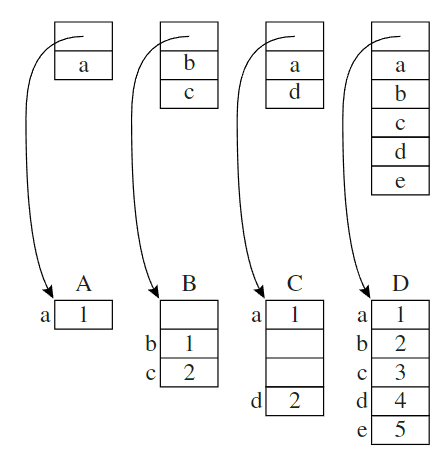
\includegraphics[width=0.22\textwidth]{pic/CP14/Field offsets in descriptors}
    \caption{Field offsets in descriptors}
    \label{fig:Field offsets in descriptors}
\end{figure}

由于类的数量远少于对象(类的实例)数量, 所以这样能节省空间. 不过这种优化导致每个 field 的具体偏移不固定了, 因此需要在运行时在 class descriptor 中动态查找(lookup) field 的真实偏移量.

\subsubsection{Method dispatch}
仍然使用图染色. 直接把 method 名混合进上述的图中, 一起染色; 也就是不仅记录 field 的偏移量, 也记录 method 的地址. 也有动态查找的开销. 

不过, 并非所有时候都可以静态知晓所有类的存在并统筹规划. 

解决方案: Hashing. 其实就是又包了一层新表, 允许通过 field/method 的名字本身索引到 field offset 或 method address. 更简单地说, 原先是 \mintinline{c++}{OffsetOrAddr[]} , 现在是 \mintinline{c++}{hashmap<Name, OffsetOrAddr>} .

\begin{itemize}
    \item Ftab(field table): field offset 或 method address (之前就有的)
    \item Ktab(key-table): 记录注册过的名字(因为有哈希冲突的问题, 需要确认名字是否真的匹配)
\end{itemize}

若要在 object $c$ 获取 field $b$, 编译器会:
\begin{enumerate}
    \item 在 $c$ 的 0 偏移处(开头)找到 class descriptor $d$.
    \item 从偏移量 $d+Ktab+hash_b$ 获取函数名 $f$
    \item 对比 $f$ 是否与 $b$ 相同
    \item 从偏移量 $d+Ftab+hash_b$ 获取 field $b$
    \item 获取 field $b$ 的内容. 
\end{enumerate}

\begin{figure}[!htb]
    \centering
    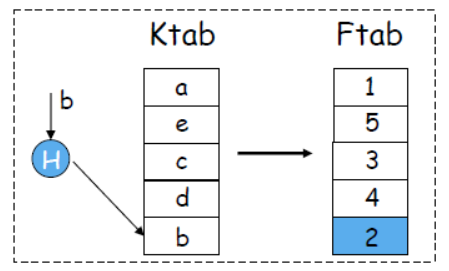
\includegraphics[width=0.309\textwidth]{pic/CP14/class descriptor}
    \caption{class descriptor}
\end{figure}


\subsection{Testing Class Membership}
每个类都是一种类型. 派生类可以看作一种 sub-type. 在进行类型转换时: 
\begin{itemize}
    \item upcast: 派生类转为基类. 永远是安全的.  在这种转换中相当于“丢失”了一些信息, upcast 后能调用/访问的 method/field 变少了. 
    \item downcast: 反之, 基类转为派生类不一定安全. 冒然转换就可能通过错误的 offset 访问到错误的、越界的内存, 很危险. 
\end{itemize}

Membership test: 为了安全的类型转换, 需要测试某个对象是否是某个类的实例. 

如何判断 $x$ 是不是类 $C$ 的实例?

朴素(慢)的做法: 递归地检查 $x$ 的 class descriptor (记作 $x.0$) 开始的继承链 $x.0$, $x.0.super$, $x.0.super.super$, $x.0.super.super.super$, $\dots$ 如果发现某个是 $C$ 的 class descriptor 则 $x$ 是 $C$ 的实例; 否则如果到最上层($\dots super==NIL$)仍未发现, 则说明不是 $C$ 的实例. 

更快的做法: display. 每个 class descriptor 储存一个 display, 也就是一个足够长(比最长继承链长)的定长列表, 记录对象的整条继承链. 就像: 
\begin{minted}{text}
    0: Object
    1: GrandparentClass
    2: ParentClass
    3: MeClass
    4: (nil)
    5: (nil)
    ...
\end{minted}
我们可以给每个类一个专属的数字 ID (例如对于 SI, 可以按照继承关系树的 BFS 序为每个类编号), 然后 display 中储存这些 ID 代表类. 由于对每个类, 其继承关系的嵌套深度在编译期已知, 因此可以立刻找到需要比较 display 中的哪一项. 例如, 假设 MeClass 的继承深度是第 3 层, 要检查 $x$ 是否为MeClass的实例, 只需检查 $x$ 的继承深度是否大于等于 3, 且 $x.0.display[3]$ 是否指向 MeClass 的 class descriptor 即可. 


\subsection{Private Fields and Methods}
private field/method: 私有的 field/method 只能被类的其他 method 访问/调用, 而不能被外部调用. 这是封装思想的体现: 调用者不该知道内部实现细节. 
通过类型检查确保私密性(privacy): 每个访问/调用处检查是否 private.

    \newpage
\section{Loop Optimizations}
\subsection{Loop in CFG}
循环在控制流图(CFG)体现为 一个节点集合 $S$, 包含 header node $h$, 并且对于 $S$ 中的任何节点 $x$:
\begin{itemize}
    \item 都有一条从 $x$ 到 $h$ 的路径
    \item 都有一条从 $h$ 到 $x$ 的路径
    \item 除了 $h$, 没有任何其他 $S$ 以外的节点能到达 $x$
\end{itemize}

\subsubsection{Dominator tree}
重要概念:
\begin{itemize}
    \item Loop entry: $h$ 是唯一一个能从外部到达的节点, 是循环的唯一入口
    \item Loop exit: 可以有多个节点能跳出循环(i.e. 后继节点不都属于 $S$)
    \item Predecessor: pred, 前驱节点
    \item Successor: succ, 后继节点
    \item Dominator: 如果 CFG 的入口节点 $s_0$ 到节点 $n$ 的所有路径都经过节点 $d$, 我们就称 $d$ 是 $n$ 的支配节点(dominator), 记作 $d \dom n$. 
    \subitem 每个节点都支配(dominate)自己
    \subitem 节点可以有多个 dominators
    \begin{figure}[!htb]
        \centering
        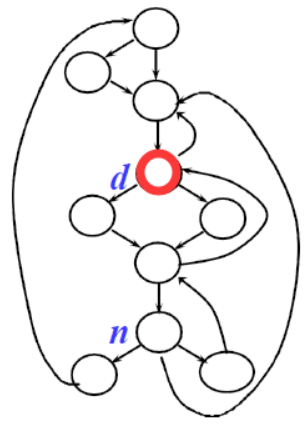
\includegraphics[width=0.16\textwidth]{pic/CP18/dominator}
        \caption{dominator}
    \end{figure}
    \subitem 求解每个节点的 dominators $D[n]$:
    \begin{itemize}
        \item 入口节点的唯一 dominator 就是自己: $D[s_0]=\{ s_0 \}$
        \item 对于其它节点: 
        \begin{align*}
            D[n]=n\cup \left( \bigcap_{p\in pred[n]} D[p] \right) \text{ for }n\ne s_0
        \end{align*}
        \item 求解过程: 一开始时令 $D[s_0]=\{ s_0 \}$, 其余节点 $D[x]=$所有节点; 然后使用上面的式子不断迭代更新直到不动点. 
    \end{itemize}
    \item Immediate dominator: 直接支配节点, 支配 $n$ 的节点中距离 $n$ 最近(但不是自己)的节点. 
    \subitem 也就是从入口结点到达 $n$ 的任何路径(不含 $n$) 中, 路径中最后一个支配 $n$ 的结点. 
    \subitem $n$ 的直接支配节点记作 $idom(n)$.
    \subitem 除了初始节点 $s_0$ 以外, 每个节点有且仅有一个直接支配节点.  可以证明, 如果 $d$ 和 $e$ 都支配 $n$, 那么要么 $d$ 支配 $e$, 要么 $e$ 支配 $d$. 因此对于某个节点 $n$ 的支配节点集合 $D[n]$, $D[n]$中的 dominators 上有全序关系. 而 $idom(n)$ 就是``最小''的那个 dominator: 不支配 $D[n]$ 中任何其他的 dominator.
    \item Dominator tree: 支配节点树
    \subitem 对于每个节点 $n$, 连接边: $idom(n)\to n$.
    \subitem 每个节点支配以自己为根的子树中的所有节点
    \begin{figure}[!htb]
        \centering
        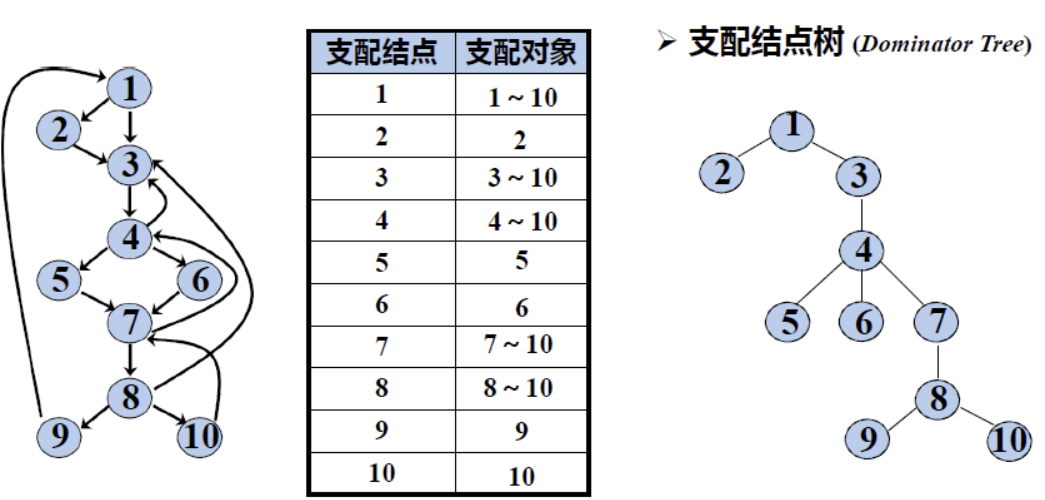
\includegraphics[width=0.42\textwidth]{pic/CP18/Dominator tree}
        \caption{Dominator tree}
    \end{figure}
\end{itemize}


\subsubsection{Natural Loop}
自然循环. 并不关心循环具体代码形式, 而是关心能否提取出易于优化的循环结构. 

如果边 $n\to h$ 满足 $h \dom n$, 则这是一个 back edge. Back edge 指向的节点 $h$ 称为 loop header.

可以基于 back edge 严谨地定义 CFG 图中的一个自然循环: 
\begin{definition}
    每个 back edge $n\to h$ 对应一个 natural loop. 这个 natural loop 中的节点集合包含一些节点 $x$ 满足: 
\begin{itemize}
    \item $h \dom x$
    \item 存在一条从 $x$ 到 $n$ 的路径不经过 $h$. 
\end{itemize}
\end{definition}


说人话就是 back edge 是从循环尾回到循环头(loop header)的边; 循环体就是中间那些被 loop header 支配的节点.  而 back edge 的意义是保证至少有一条路径能返回首节点 $h$. 

可以有多个 back edge 对应一个 natural loop: 例如 for 语句中的每个 continue 都给这个 natural loop 新增了一个 back edge.

注:
\begin{itemize}
    \item 循环可以嵌套, 可以共享首节点.
    \item 除了共享首节点的情况外, 两个循环要么完全不相交, 要么一个完全嵌入另一个(或者说后者包含前者). 
    \item 最内循环(innermost loop): 最里的循环, 不包含其他循环(不被其他循环嵌入). 
\end{itemize}

\begin{figure}[!htb]
    \centering
    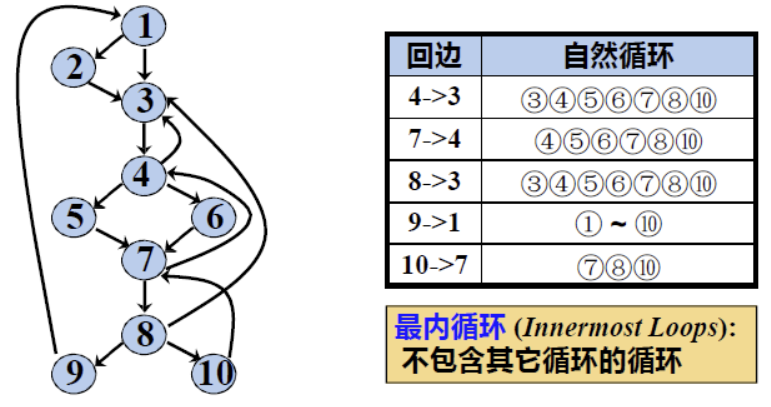
\includegraphics[width=0.309\textwidth]{pic/CP18/innermost loop}
    \caption{innermost loop}
\end{figure}


\subsubsection{Loop-nest Tree}
表达循环的嵌套关系. 树中每个节点对应一个 loop header 及其对应的 natural loops 节点集合. 如果这个 loop heder 对应多个 natural loops (共享首节点), 也合并到同一个节点. 

\begin{figure}[!htb]
    \centering
    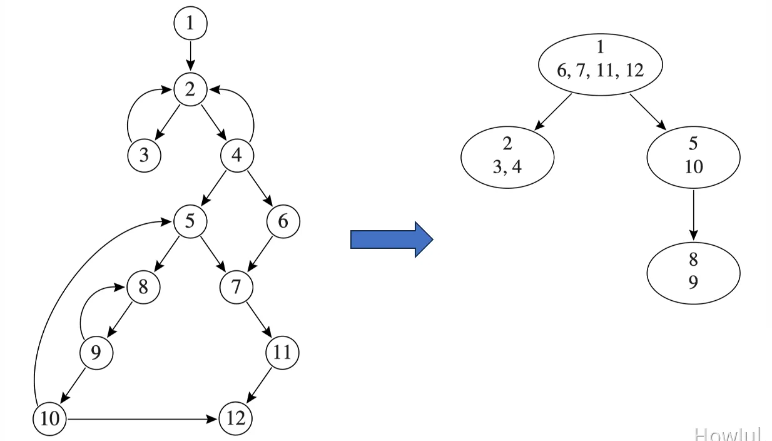
\includegraphics[width=0.42\textwidth]{pic/CP18/Loop-nest Tree}
    \caption{Loop-nest Tree}
\end{figure}
节点的上半部分表示该节点对应的 loop header. 可以把整个 procedure 视为在一个假想的大循环中, 作为树的根节点. 叶节点即对应最内循环. 

Loop preheader: 前置首节点. 许多优化操作会在进入循环前进行一些准备工作, 也就是在紧挨着循环头之前插入一些语句. 因此我们可以在 loop header 之前插入一个 loop preheader 用来安置这些语句. 
\begin{itemize}
    \item loop preheader 的唯一后继就是 loop header
    \item 循环 $L$ 外到达首节点的边 $x\to h$ 改为进入前置首节点: $x\to p$
    \item 循环 $L$ 里到达首节点的边不变
\end{itemize}

\begin{figure}[!htb]
    \centering
    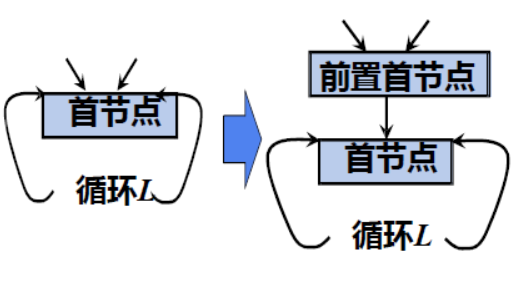
\includegraphics[width=0.309\textwidth]{pic/CP18/Loop preheader}
    \caption{Loop preheader}
\end{figure}


\subsection{Loop Invariant Hoisting}
循环不变代码外提. 

Loop-invariant: 如果某个表达式的值在循环中不会改变, 对循环来讲是固定值, 则称表达式 loop-invariant. 显然, 所有常数都 loop-invariant. 

赋值语句 $x := v_1\text{ OP }v_2$  是 invariant 的当且仅当其操作数 $v_1$ 和 $v_2$ 都满足: 
\begin{itemize}
    \item 操作数是常数, 或是
    \item 对于操作数中使用到的变量, 其 def 都在循环外, 或是
    \item 对于操作数中使用到的变量, 在执行赋值语句时其 def 唯一, 且 loop-invariant.
\end{itemize}
说人话就是操作数及其使用的变量也得 loop-invariant, 而且不能在循环中因为控制流跳转等原因导致变量 def 不唯一. 

可以归纳地检查赋值语句 $x := v_1\text{ OP }v_2$ 的操作数是否 invariant:
\begin{itemize}
    \item Base cases:
    \subitem 常数: 一定是 invariant 的. 
    \subitem 变量的 use: 该变量所有 defs 都在循环外则 invariant.
    \item Inductive cases:
    \subitem 表达式: 多个 invariant 表达式进行运算仍然 invariant.
    \subitem 变量的 use: 要求在执行该语句时只可能有唯一的 def 有效, 且这个 def 的右侧(RHS) 是 loop-invariant 的. 
\end{itemize}

优化: 这样的表达式在循环外就可以求值, 而非每轮循环都计算一次. 这就是 loop-invariant code motion.
\begin{itemize}
    \item Code hoisting: 如果这样的表达式在循环中需要使用, 则可以将求值提升到循环开始前. 
    \item Code sinking: 如果这样的表达式在循环结束后需要使用, 则可以将求值下沉到循环结束后. 
\end{itemize}

注意表达式的值是 loop-invariant 的不代表 hoisting 就是合法的: 归根结底, 这相当于只关心了 表达式 的值, 但忽视了其副作用; 盲目上提会破坏代码的语义(semantics)信息. 

\subsubsection{Code hoisting}
hoisting 的判据: 当且仅当满足如下所有条件时可以提升形如 $t := a\text{ OP }b$ 的赋值语句(赋值语句就是 def)$d$:
\begin{itemize}
    \item $d$ 必须支配所有 $t$ 在其上 live-out 的循环出口(loop exits).
    \item 在循环中 $t$ 只能有唯一的 def.
    \item $t$ 不属于 loop preheader 的 live-out 集合; 换句话说, $t$ 在进入循环前不是活跃的. 
\end{itemize}


如果这个赋值语句有一定的副作用, 那么上述规则就不足够, 需要添加更多判断、约束. 

将 while 转写为 for 有助于优化: 拷贝一份条件判断块到循环体末尾即可. 这是由于 while 特殊的控制流结构可能会导致判据中最后一条要求无人能达到, 要把 while 转化为刚刚研究的 repeat-until 这种模式的 natural loops.

\begin{figure}[!htb]
    \centering
    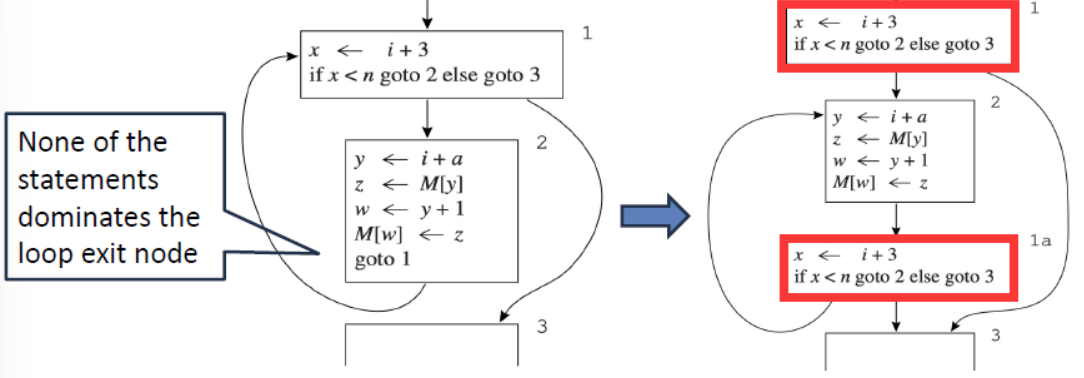
\includegraphics[width=0.42\textwidth]{pic/CP18/while}
    \caption{while}
\end{figure}




    % https://cs.nju.edu.cn/changxu/2_compiler/index.html
    % https://pku-minic.github.io/online-doc/#/preface/
    % https://syuanz.wiki/accipit/
\end{document}